\documentclass{article}
\usepackage{ctex}

\title{数字逻辑与计算机组成\\ {\small 实验 5: 存储器及数据通路设计
}}
\author{王卫东\quad 221900332}
\date{\zhtoday}

\usepackage{hyperref}
\usepackage{algorithm}
\usepackage{algorithmicx}
\usepackage{algpseudocode}
\usepackage{float}  
\usepackage{lipsum}
\usepackage{color, xcolor}
\usepackage{listings}
\usepackage{dirtree}
\usepackage{ulem}
\usepackage{graphicx}
\usepackage{amsmath}
\usepackage{amssymb}
\usepackage{amsfonts}
\usepackage{xcolor}
\usepackage{tikz}
\usepackage{multirow}
\usepackage{zhnumber} % change section number to chinese
\renewcommand\thesection{\zhnum{section}}
\renewcommand\thesubsection{\arabic{subsection}}
\usetikzlibrary{arrows,shapes,chains}

\begin{document}
    \maketitle

    \section{实验目的}

    \begin{enumerate}
        \item 理解存储器 RAM 和 ROM 的读写方法,掌握支持 RV32I 存取指令的数据存储器设计方法。
        \item 理解处理器读取指令的过程,掌握 RV32I 下取指令部件设计方法。
        \item 理解 RV32I 运算指令功能,掌握指令译码、取操作数、运算、访存等执行不同阶段的实现方法。
        \item 理解 RV32I 每条目标指令的功能和对应数据通路的关系,掌握单周期数据通路的设计方法。
    \end{enumerate}
    \section{实验环境}

    Logisim:https://github.com/Logisim-Ita/Logisim
    RISC-V 模拟器工具 RARS:https://github.com/thethirdone/rars

    \section{实验内容}
    
    \subsection{数据存储器}

    \subsubsection{整体方案设计}
    \begin{figure}[H]
    \centering
    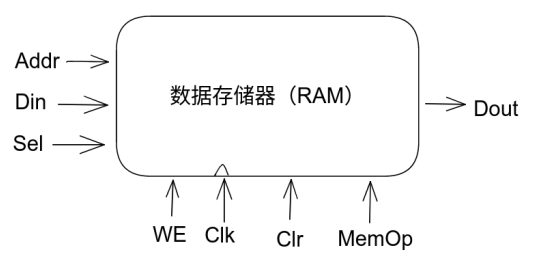
\includegraphics[width=0.4\textwidth]{1.1.png}
    \caption{数据存储器整体方案设计}
    \end{figure}

    \subsubsection{顶层模块设计}
    实验电路较为简单,不需要顶层模块设计图。

    \subsubsection{引脚作用}
    \begin{table}[H]
    \centering
    \begin{tabular}{|c|c|}
        \hline
        Addr[15:0]  & 输入的地址 \\ \hline
        Din[31:0] & 输入的需要存储的数据 \\ \hline
        Sel   & 输入的片选信号 \\ \hline
        WE   & 输入的写使能信号 \\ \hline
        Clk   & 输入的时钟,上升沿有效 \\ \hline
        MemOp[2:0]   & 输入的存取模式选择信号 \\ \hline
        Dout[31:0]   & 输出的读取的数据 \\ \hline
    \end{tabular}
    \caption{数据存储器引脚作用}
    \end{table}
    MemOp[2:0] 为存取模式选择信号,其值和对应的存取模式如下图所示。
    \begin{figure}[H]
    \centering
    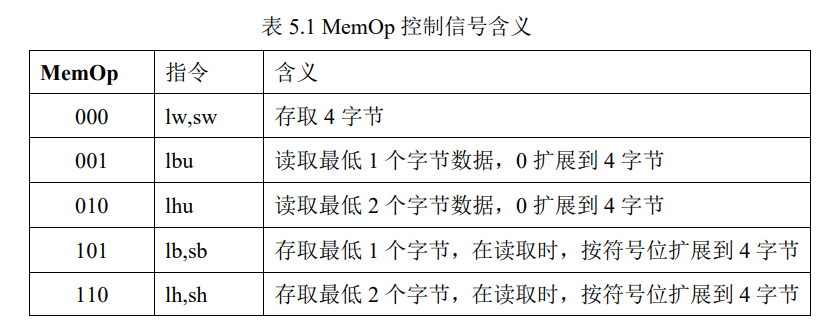
\includegraphics[width=0.4\textwidth]{1.2.png}
    \caption{MemOp[2:0] 与存取模式对应关系}
    \end{figure}

    \subsubsection{原理图和电路图}
    原理图略,使用4个8位 RAM 来实现可以读取字、半字、字节的存储器。

    \begin{figure}[H]
    \centering
    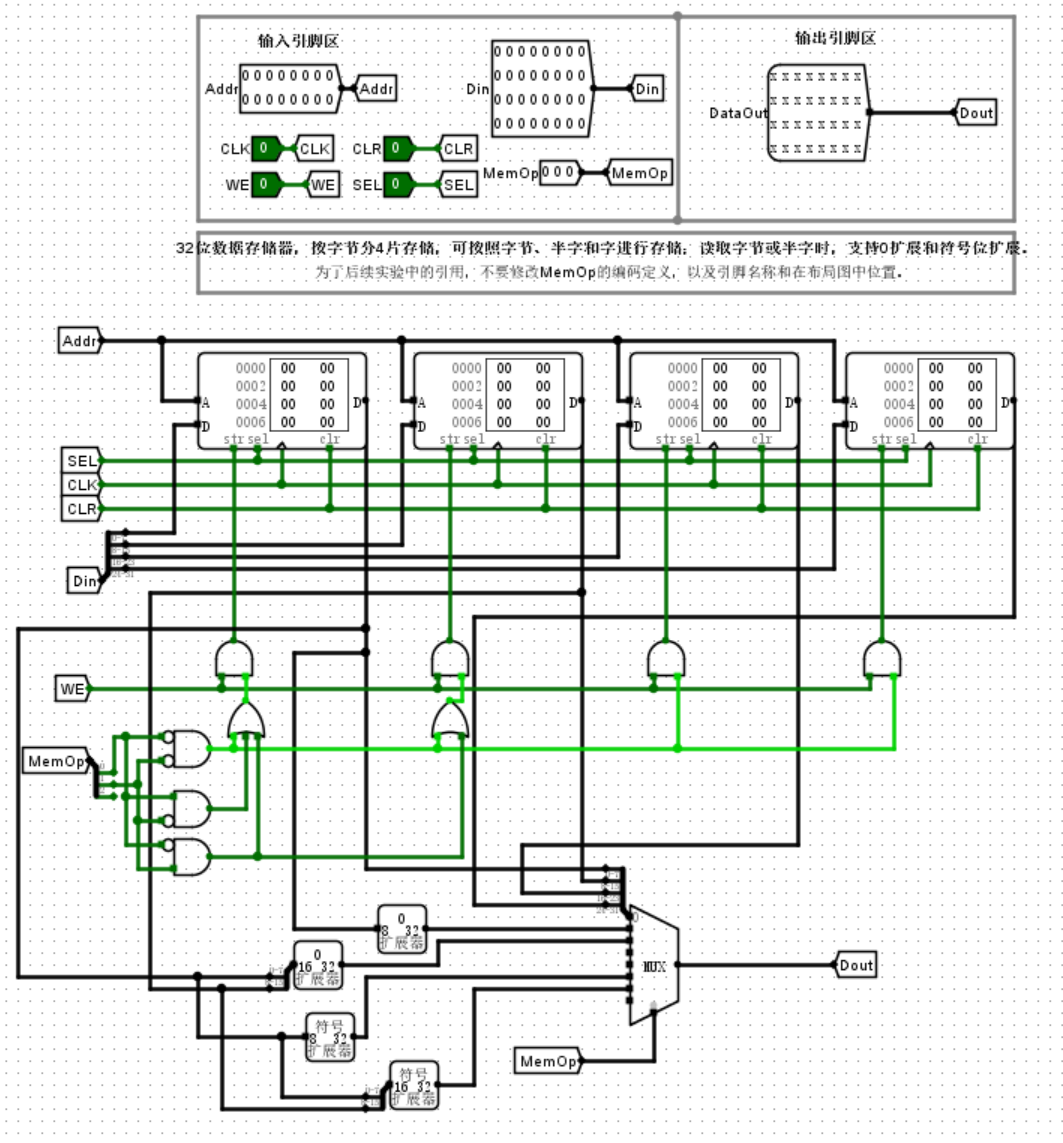
\includegraphics[width=0.8\textwidth]{1.4.2.png}
    \caption{数据存储器电路图}
    \end{figure}

    \subsubsection{仿真测试图}
    \begin{figure}[H]
    \centering
    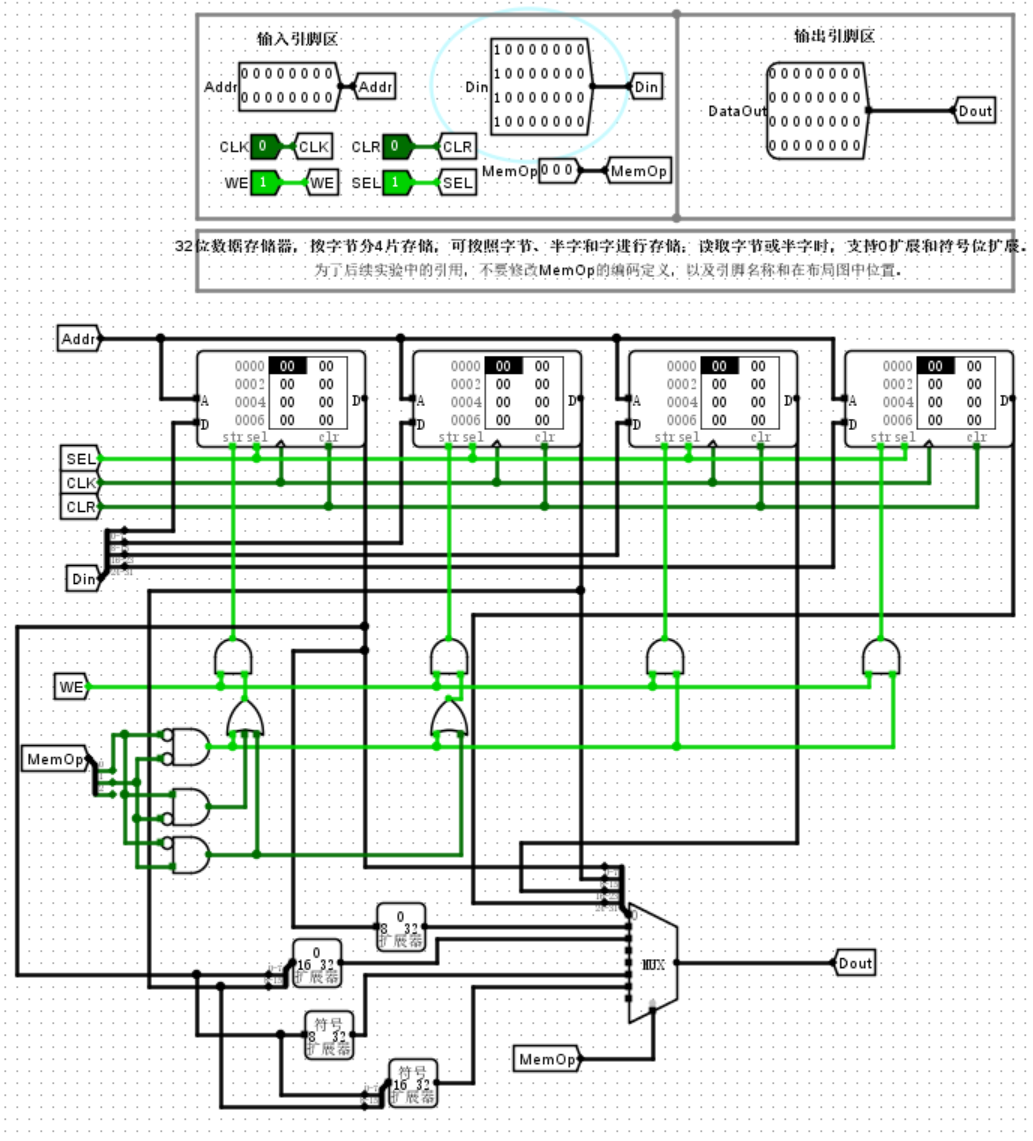
\includegraphics[width=0.4\textwidth]{1.5.1.png}
    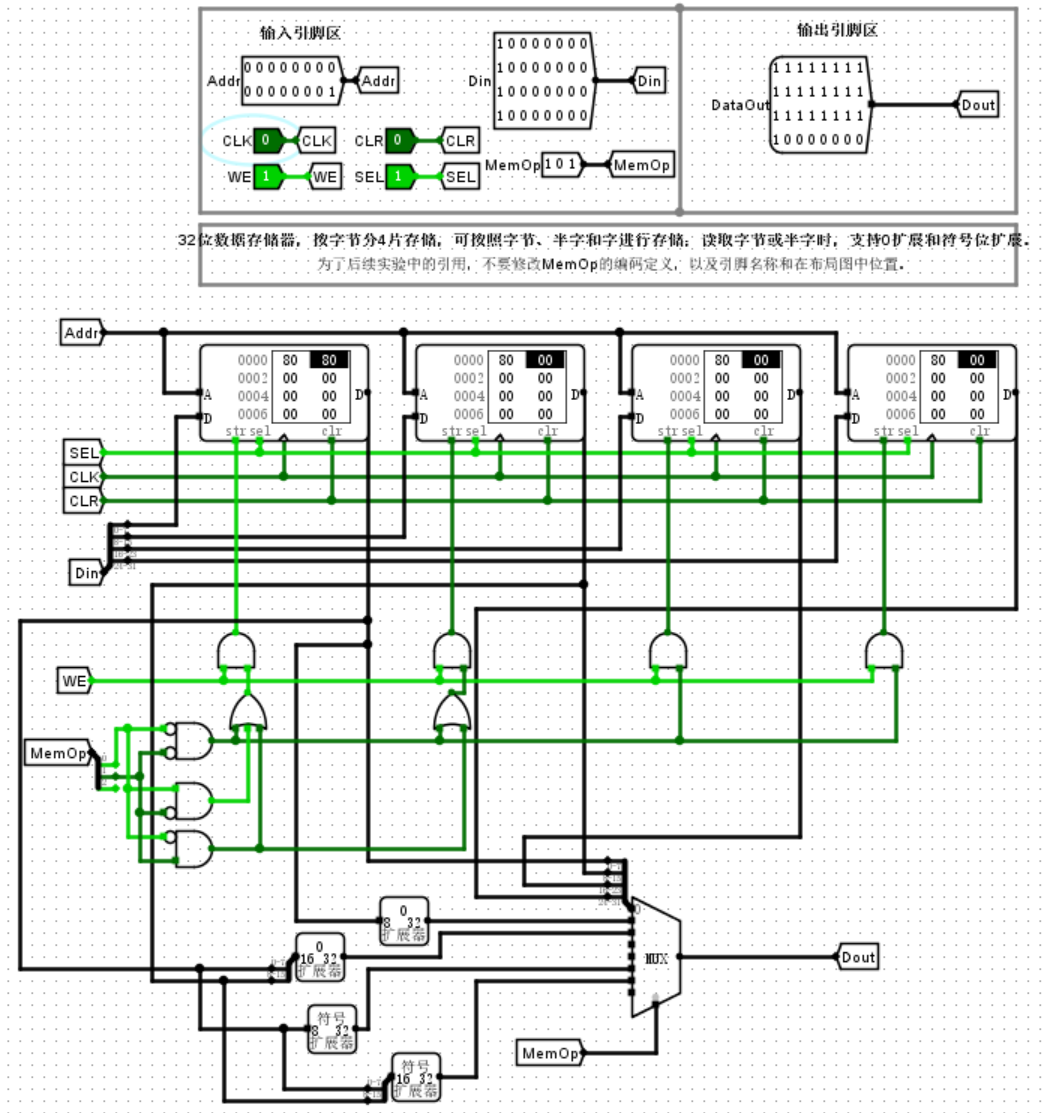
\includegraphics[width=0.4\textwidth]{1.5.2.png}
    
    \caption{数据存储器仿真测试图}
    \end{figure}

    \begin{figure}[H]
    \centering
    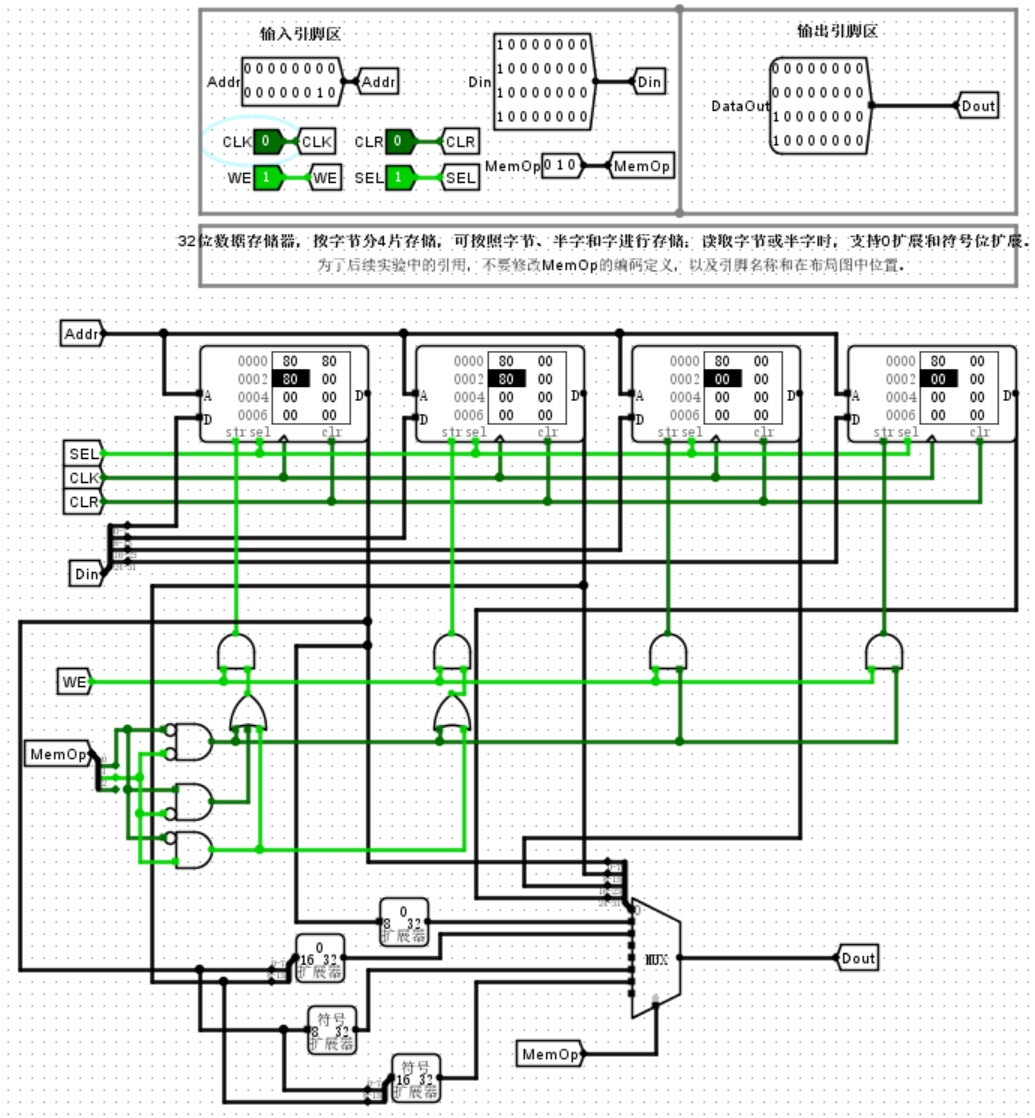
\includegraphics[width=0.4\textwidth]{1.5.3.png}  
    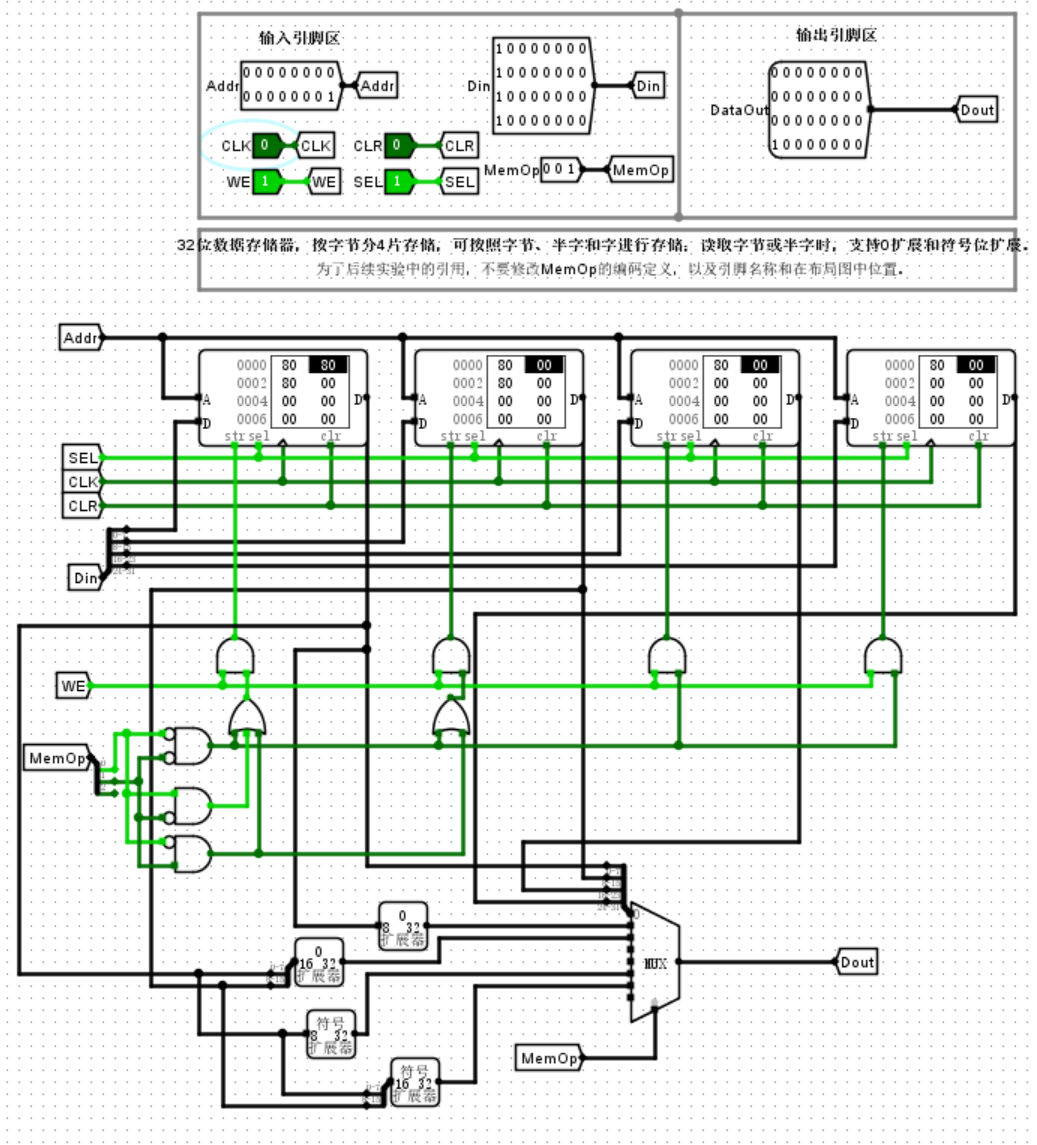
\includegraphics[width=0.4\textwidth]{1.5.4.png}
    \caption{数据存储器仿真测试图}
    \end{figure}
    图 1 在 0x0 号地址处存储了 4 字节,使得四个 RAM 中的数据均为 0x80;图 2 在 0x1 号地址存储了最低 1 字节,使得最低 1 字节对应的 RAM 中的数据为 0x80,其他为 0;图 3 在 0x2 号地址存储了最低 2 字节,使得最低 2 字节对应的 RAM 中的数据为 0x80,其他为 0;图 4 读取了 0x1 号地址的最低 1 字节数据并零扩展为4字节。以上模拟结果均正确。
    
    

    \subsubsection{错误现象及分析}
    在完成实验的过程中,没有遇到任何错误。

    \subsection{ASCII 码显示}

    \subsubsection{整体方案设计}
    \begin{figure}[H]
    \centering
    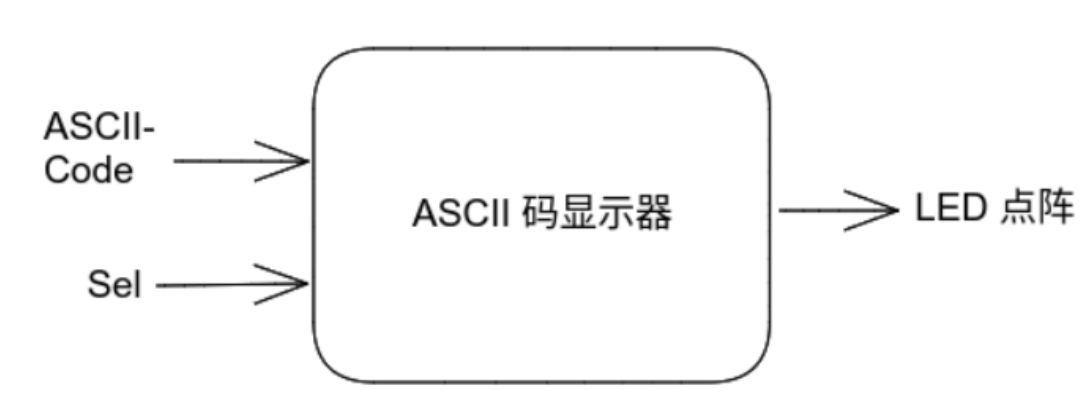
\includegraphics[width=0.4\textwidth]{2.1.png}
    \caption{ASCII 码显示整体方案设计}
    \end{figure}

    \subsubsection{顶层模块设计}
    实验电路较为简单,不需要顶层模块设计图。

    \subsubsection{引脚作用}
    \begin{table}[H]
    \centering
    \begin{tabular}{|c|c|}
        \hline
        ASCII-Code[7:0]   & 输入的 ASCII 码 \\ \hline
        Sel   & 输入的片选信号 \\ \hline
        LED 点阵   & 输出的 LED 点阵显示 \\ \hline
    \end{tabular}
    \caption{ASCII 码显示引脚作用}
    \end{table}

    \subsubsection{原理图和电路图}
    原理图略,观察到点阵文件中每一行 16 个字节表示一个字符的ASCII 码显示,即为4位0+8位ASCII码+4位LED里的行数。因为需要同时显示所有行,用 16 个内容相同的 ROM 实现。

    \begin{figure}[H]
    \centering
    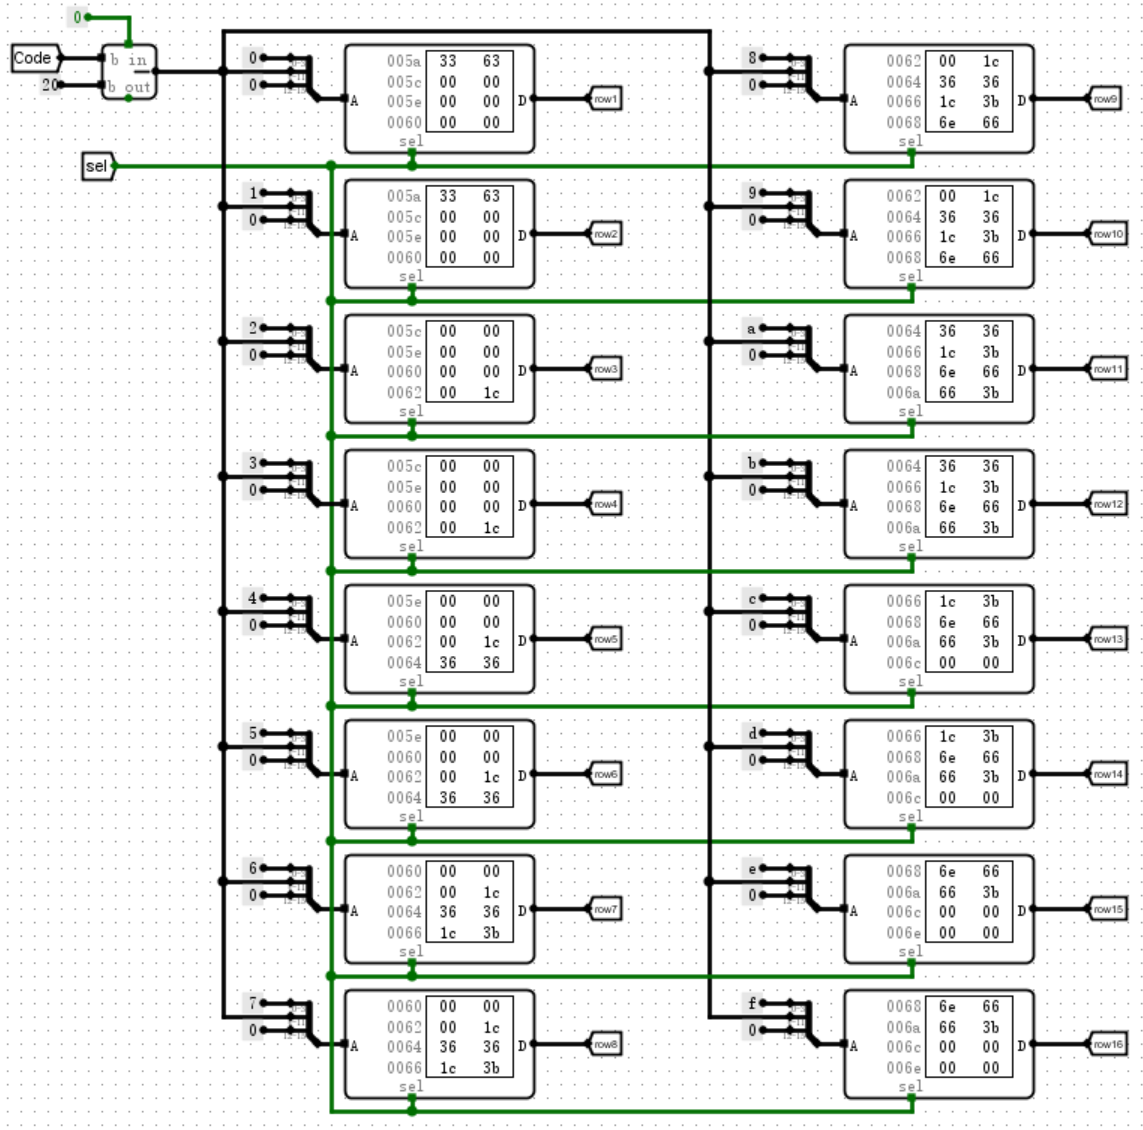
\includegraphics[width=0.8\textwidth]{2.4.2.png}
    \caption{ASCII 码显示电路图}
    \end{figure}

    \subsubsection{仿真测试图}
    \begin{figure}[H]
    \centering
    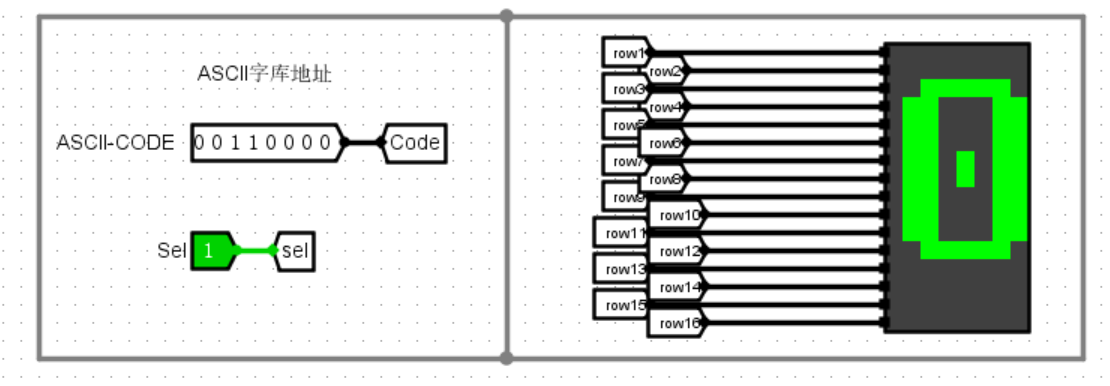
\includegraphics[width=0.4\textwidth]{2.5.1.png}
    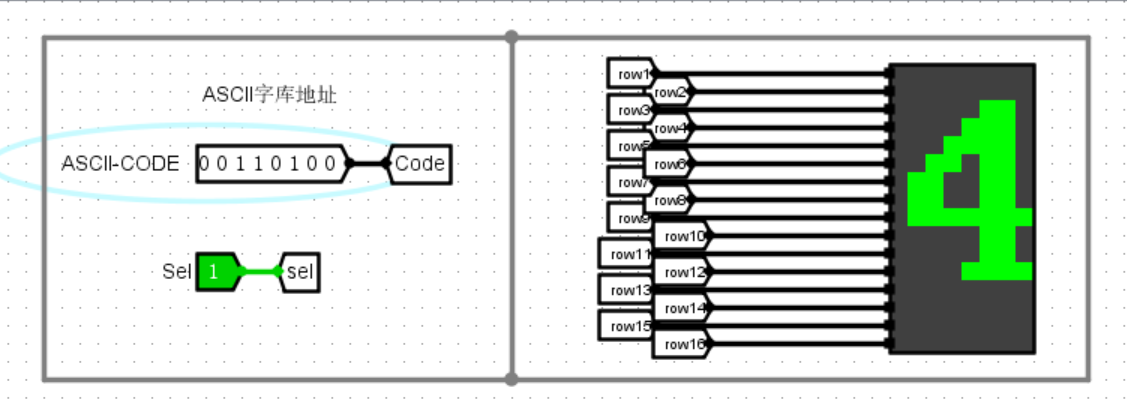
\includegraphics[width=0.4\textwidth]{2.5.2.png}
        
    \caption{ASCII 码显示仿真测试图}
    \end{figure}

    \begin{figure}[H]
    \centering
    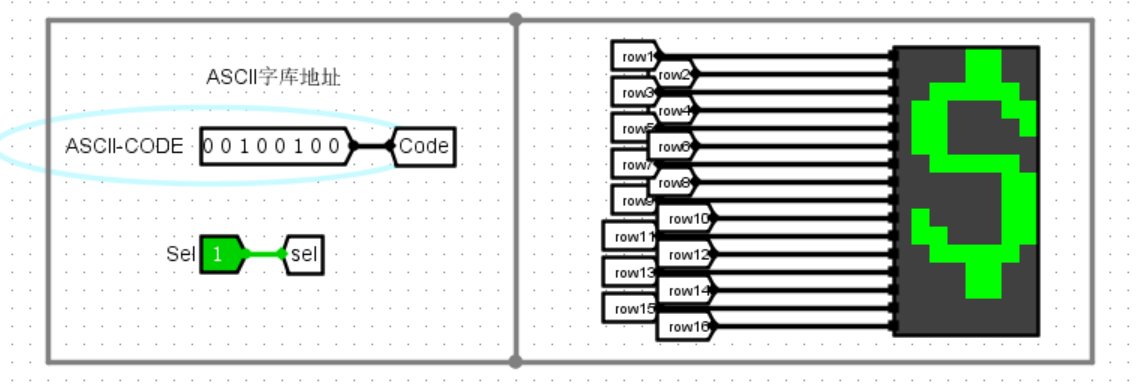
\includegraphics[width=0.4\textwidth]{2.5.3.png}
    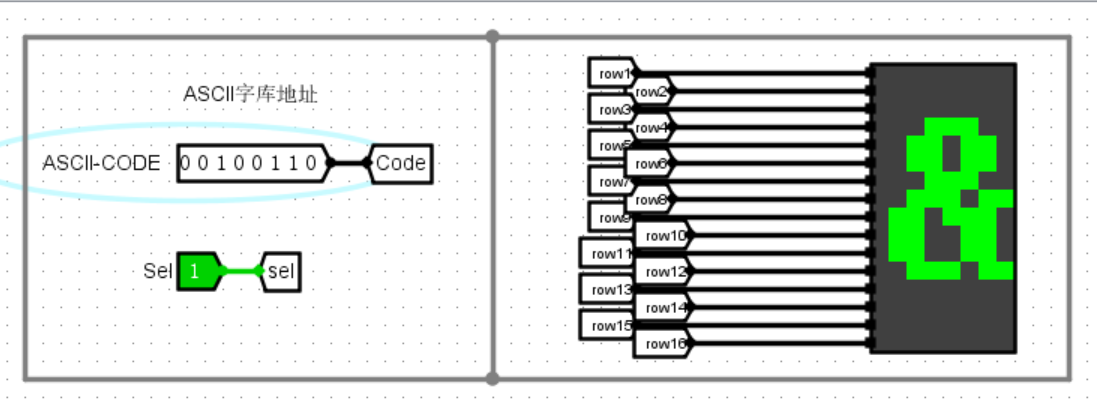
\includegraphics[width=0.4\textwidth]{2.5.4.png}
    \caption{ASCII 码显示仿真测试图}
    \end{figure}
    如图所示。

    \subsubsection{错误现象及分析}
    在完成实验的过程中,没有遇到任何错误。

    \subsection{取指令部件 IFU}

    \subsubsection{整体方案设计}
    \begin{figure}[H]
    \centering
    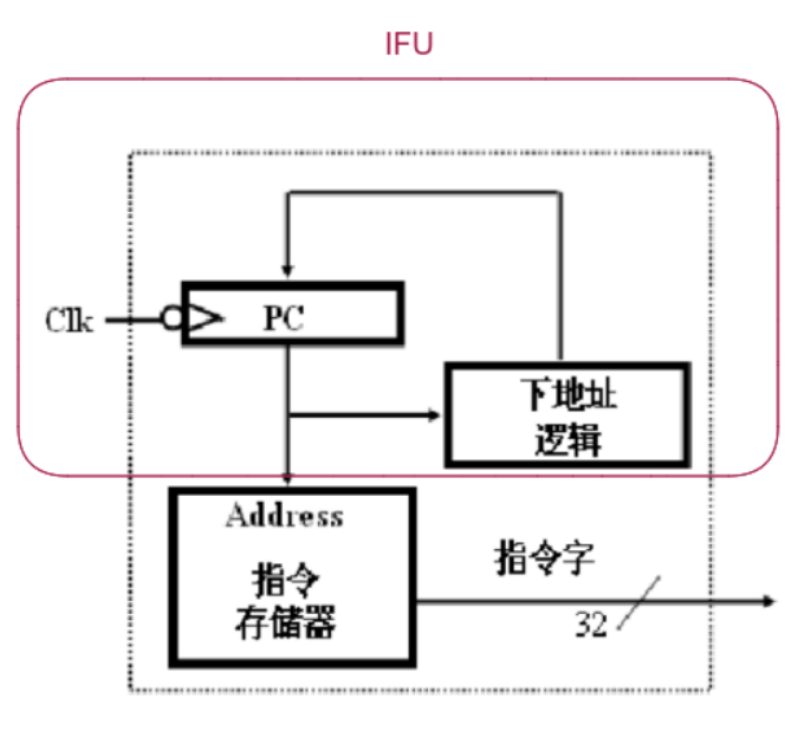
\includegraphics[width=0.4\textwidth]{3.1.png}
    \caption{取指令部件 IFU 整体方案设计}
    \end{figure}

    \subsubsection{顶层模块设计}
    实验电路较为简单,不需要顶层模块设计图。

    \subsubsection{引脚作用}
    \begin{table}[H]
    \centering
    \begin{tabular}{|c|c|}
        \hline
        Init Addr[31:0]   & 输入的初始地址,在复位 Reset 按下时同步赋给 PC \\ \hline
        Imm[31:0]    & 输入的当前指令的立即数 \\ \hline
        BusA[31:0]  & 输入的总线 A 数据 \\ \hline
        Clk  & 输入的时钟信号(上升沿有效) \\ \hline
        Reset  & 输入的复位信号 \\ \hline
        PC[31:0]  & 输出的程序计数器的值 \\ \hline
        Halt   & 输入的终止信号,指示程序已经终止 \\ \hline
        NxtAsrc  & 输入的下地址逻辑中加法器 A 端 MUX 控制信号 \\ \hline
        NxtBsrc  & 输入的下地址逻辑中加法器 B 端 MUX 控制信号 \\ \hline
    \end{tabular}
    \caption{取指令部件 IFU 引脚作用}
    \end{table}

    \subsubsection{原理图和电路图}

    \begin{figure}[H]
    \centering
    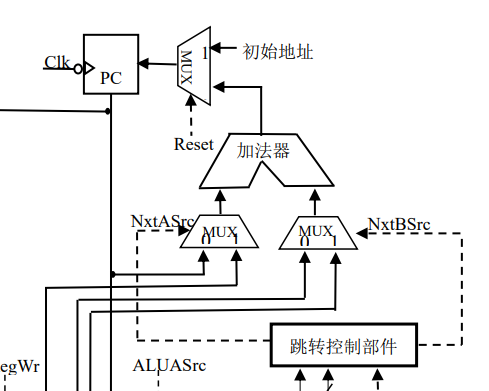
\includegraphics[width=0.8\textwidth]{3.4.1.png}
    \caption{取指令部件 IFU 原理图}
    \end{figure}

    \begin{figure}[H]
    \centering
    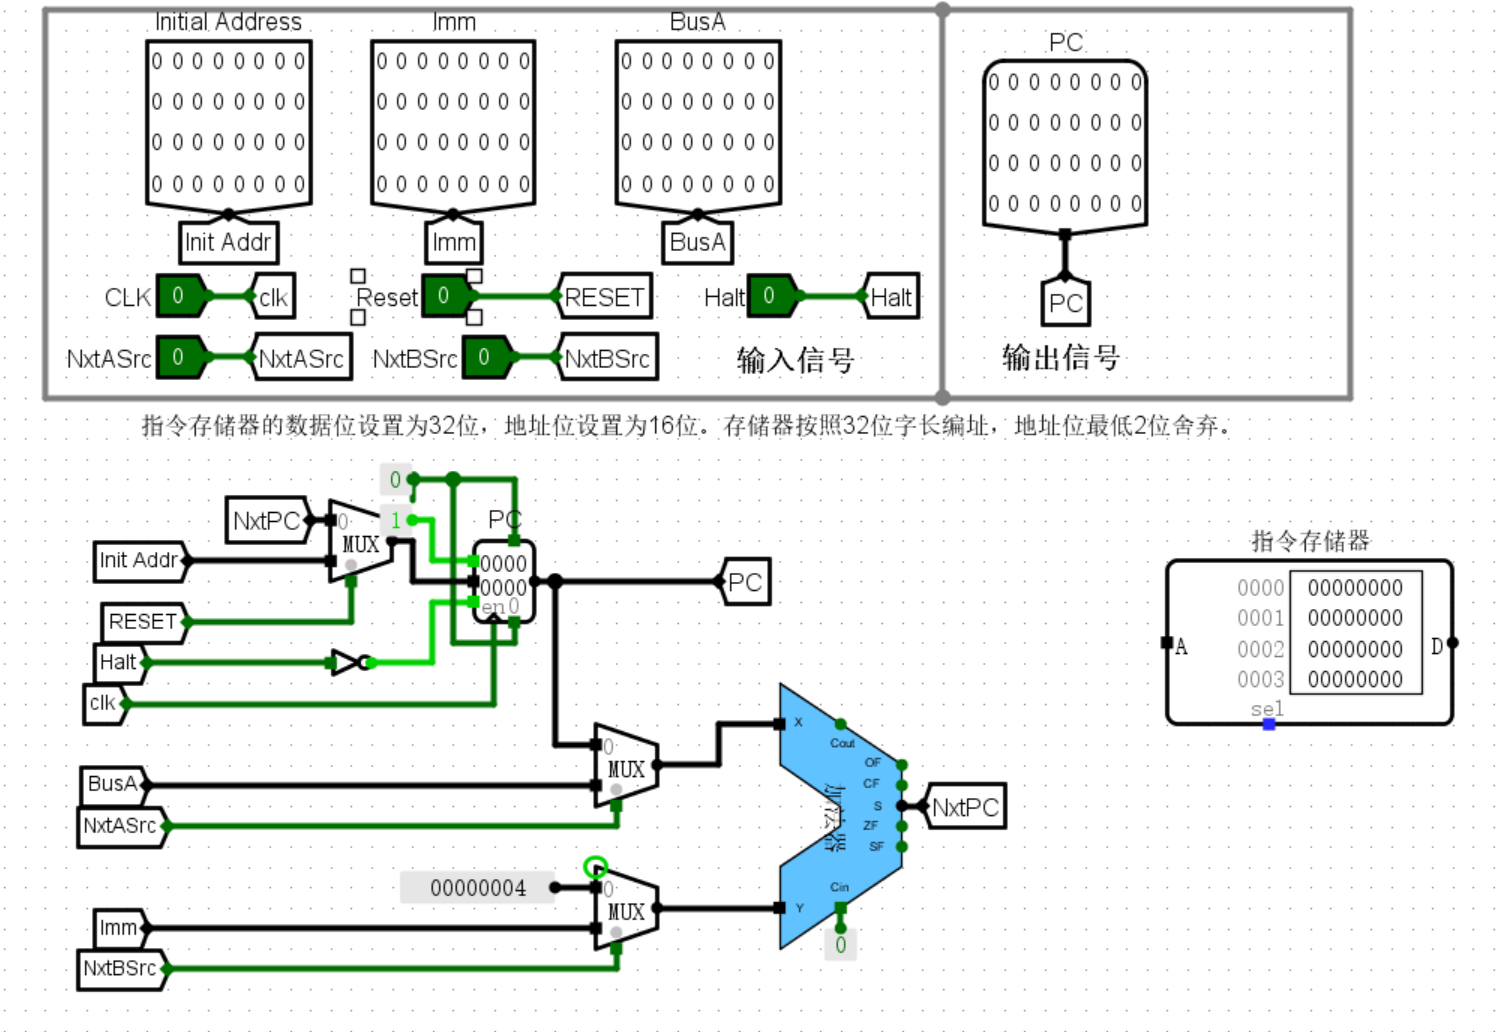
\includegraphics[width=0.8\textwidth]{3.4.2.png}
    \caption{取指令部件 IFU 电路图}
    \end{figure}

    \subsubsection{仿真测试图}
    \begin{figure}[H]
    \centering
    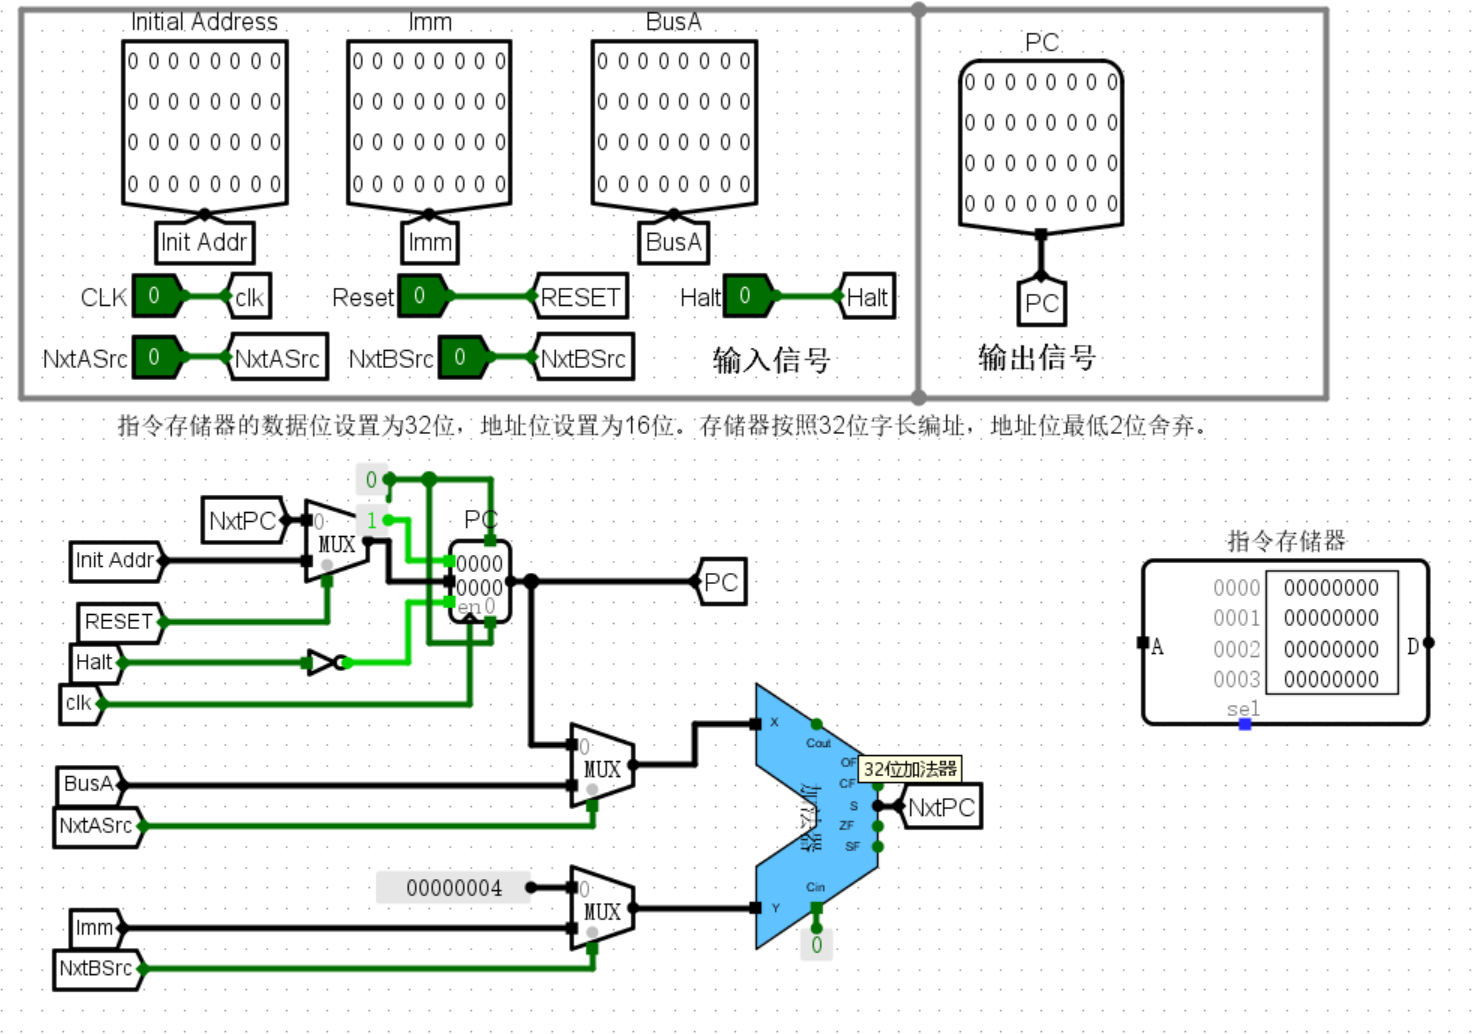
\includegraphics[width=0.8\textwidth]{3.5.1.png}
    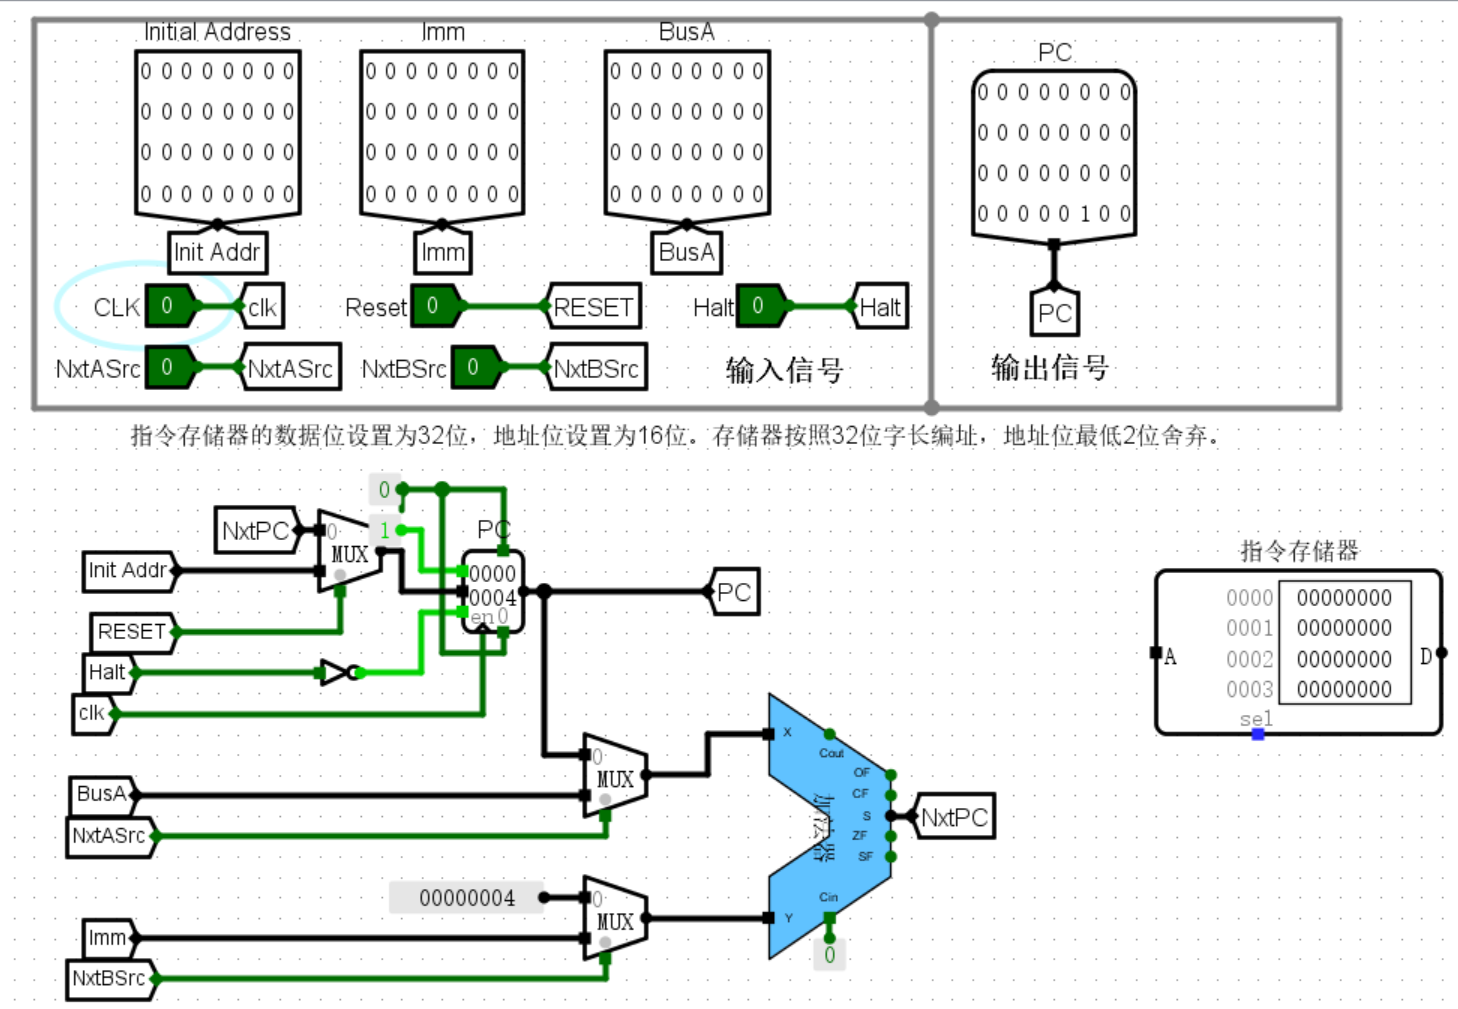
\includegraphics[width=0.8\textwidth]{3.5.2.png}
    \caption{取指令部件 IFU 仿真测试图}
    \end{figure}
    
    \begin{figure}[H]
        \centering
        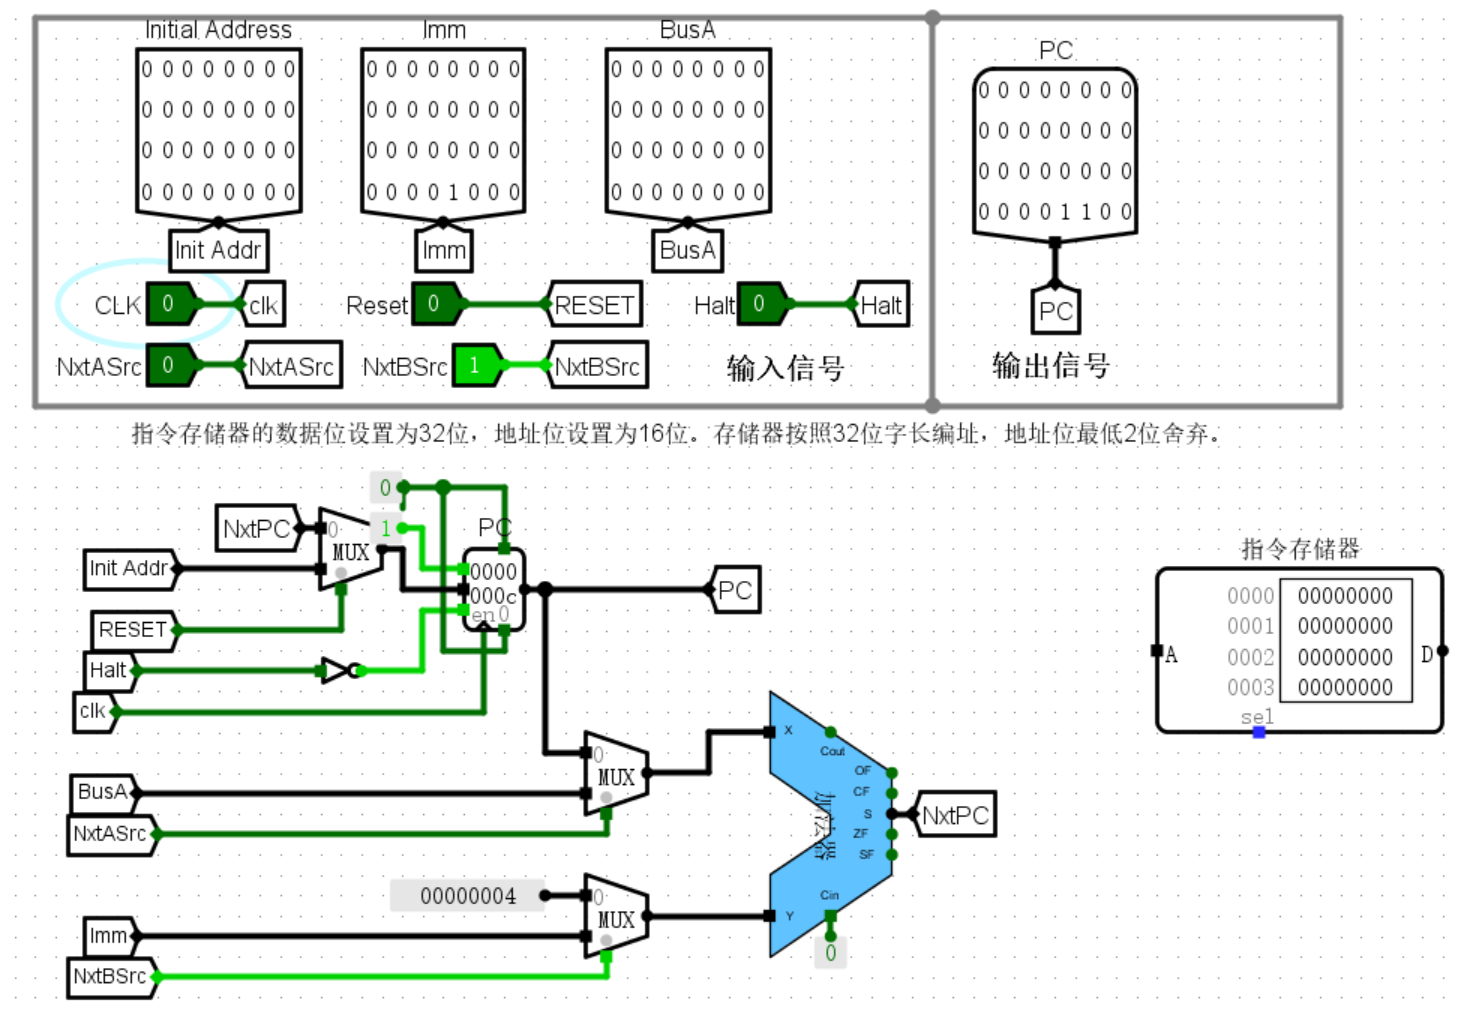
\includegraphics[width=0.8\textwidth]{3.5.3.png}
        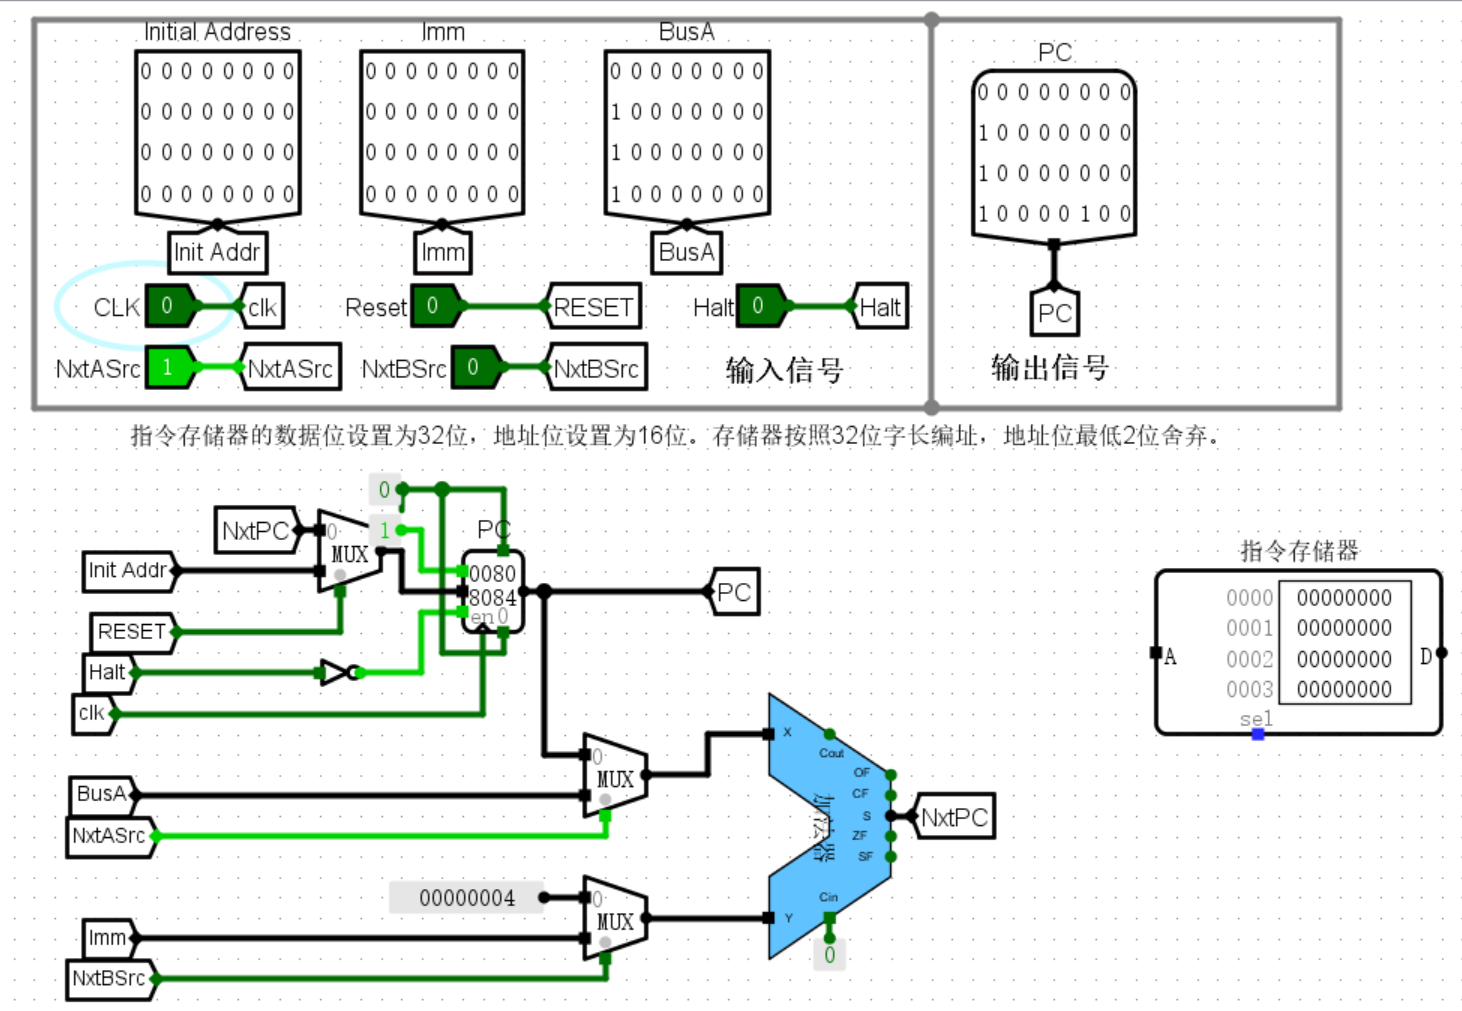
\includegraphics[width=0.8\textwidth]{3.5.4.png}
        \caption{取指令部件 IFU 仿真测试图}
    \end{figure}
    初始情况如图 1 所示。将 NxtAsrc 和 NxtBsrc 均设为 0,PC 初始值为 0。此时的次态方程是$PC* = PC + 4$。一个周期后,PC 的值变为 4,如图 2 所示。将 NxtBsrc 设为 1,Imm 设为 8。此时的次态方程为 $PC* = PC + Imm$。一个周期后,PC 的值变为 12,如图 3 所示。将 NxtAsrc 设为 1,NxtBsrc 设为 0,BusA 设为 0x00808080。此时的次态方程为 $PC* = BusA + 4$。一个周期后,PC 的值变为 0x00808084,如图 4 所示。所有仿真结果与预期相符。
    
    \subsubsection{错误现象及分析}
    在完成实验的过程中,没有遇到任何错误。

    \subsection{立即数扩展器}
    \subsubsection{整体方案设计}
    \begin{figure}[H]
    \centering
    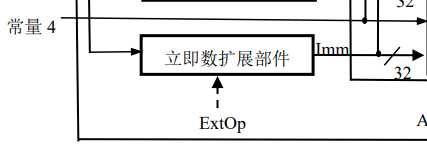
\includegraphics[width=0.4\textwidth]{4.1.png}
    \caption{立即数扩展器整体方案设计}
    \end{figure}

    \subsubsection{顶层模块设计}
    实验电路较为简单,不需要顶层模块设计图。

    \subsubsection{引脚作用}
    \begin{table}[H]
    \centering
    \begin{tabular}{|c|c|}
        \hline
        Instr[31:0]     & 输出的扩展后的立即数 \\ \hline
        Imm[31:0]   & 输出的立即数 \\ \hline
        ExtOp[2:0] & 输入的立即数扩展方式 \\ \hline
    \end{tabular}
    \caption{立即数扩展器引脚作用}
    \end{table}

    \begin{table}[H]
        \centering
        \begin{tabular}{|c|c|}
            \hline
            ExtOp[2:0]  & 扩展方式 \\ \hline
            0   & I-type \\ \hline
            1   & U-type \\ \hline
            2 & S-type \\ \hline
            3 & B-type \\ \hline
            4 & J-type \\ \hline
        \end{tabular}
        \caption{立即数扩展器引脚作用}
    \end{table}

    \subsubsection{原理图和电路图}
    原理图略,主要思想是使用分线器和扩展器对立即数进行合理的拼接。


    \begin{figure}[H]
    \centering
    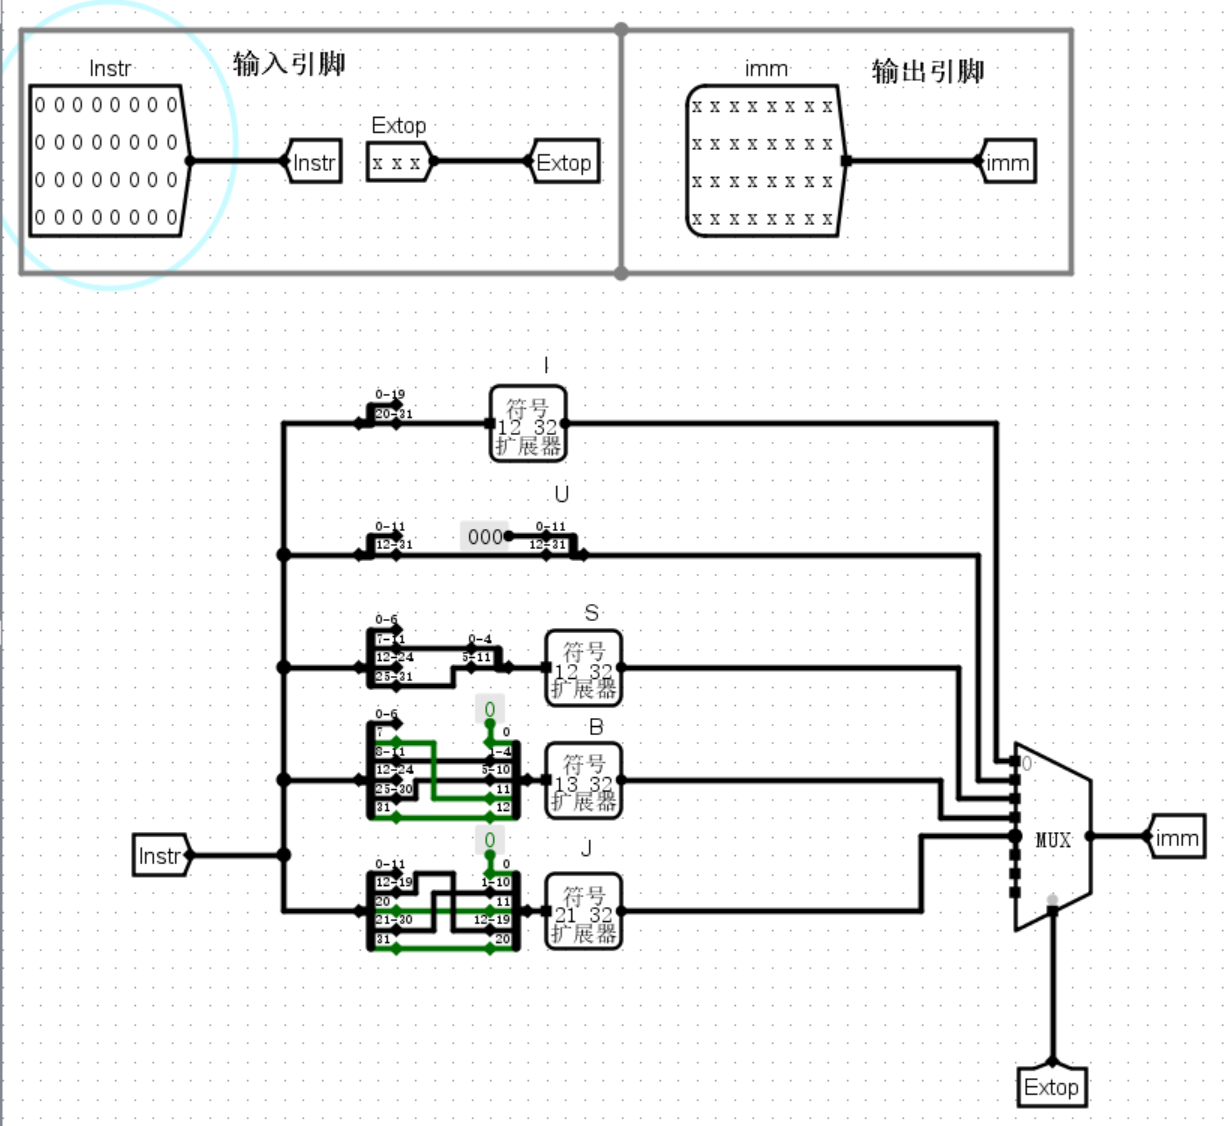
\includegraphics[width=0.8\textwidth]{4.4.2.png}
    \caption{立即数扩展器电路图}
    \end{figure}

    \subsubsection{仿真测试图}
    \begin{figure}[H]
    \centering
    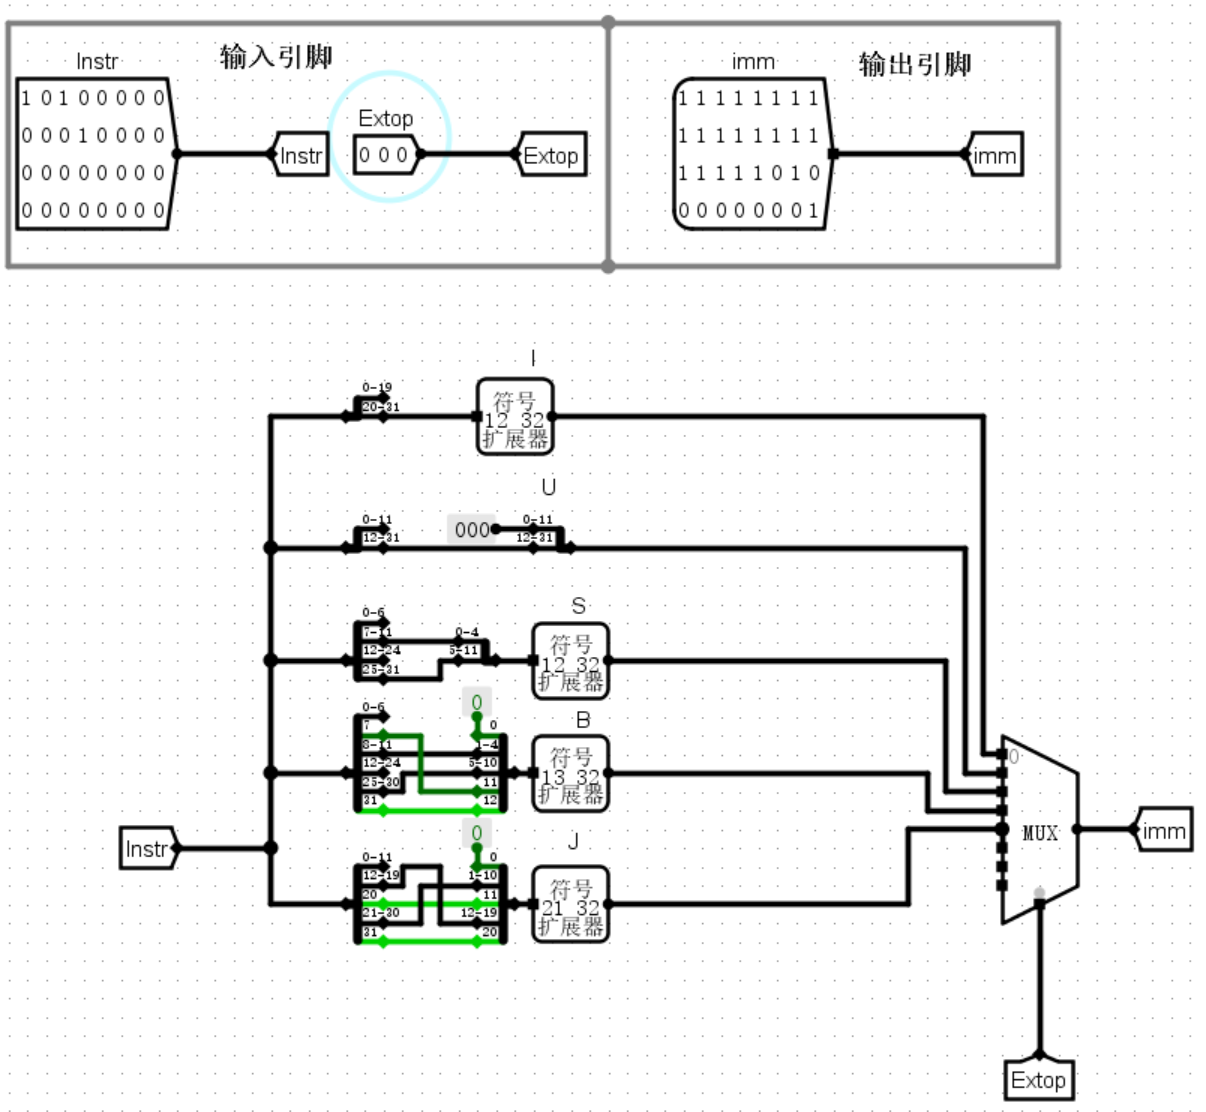
\includegraphics[width=0.8\textwidth]{4.5.1.png}
    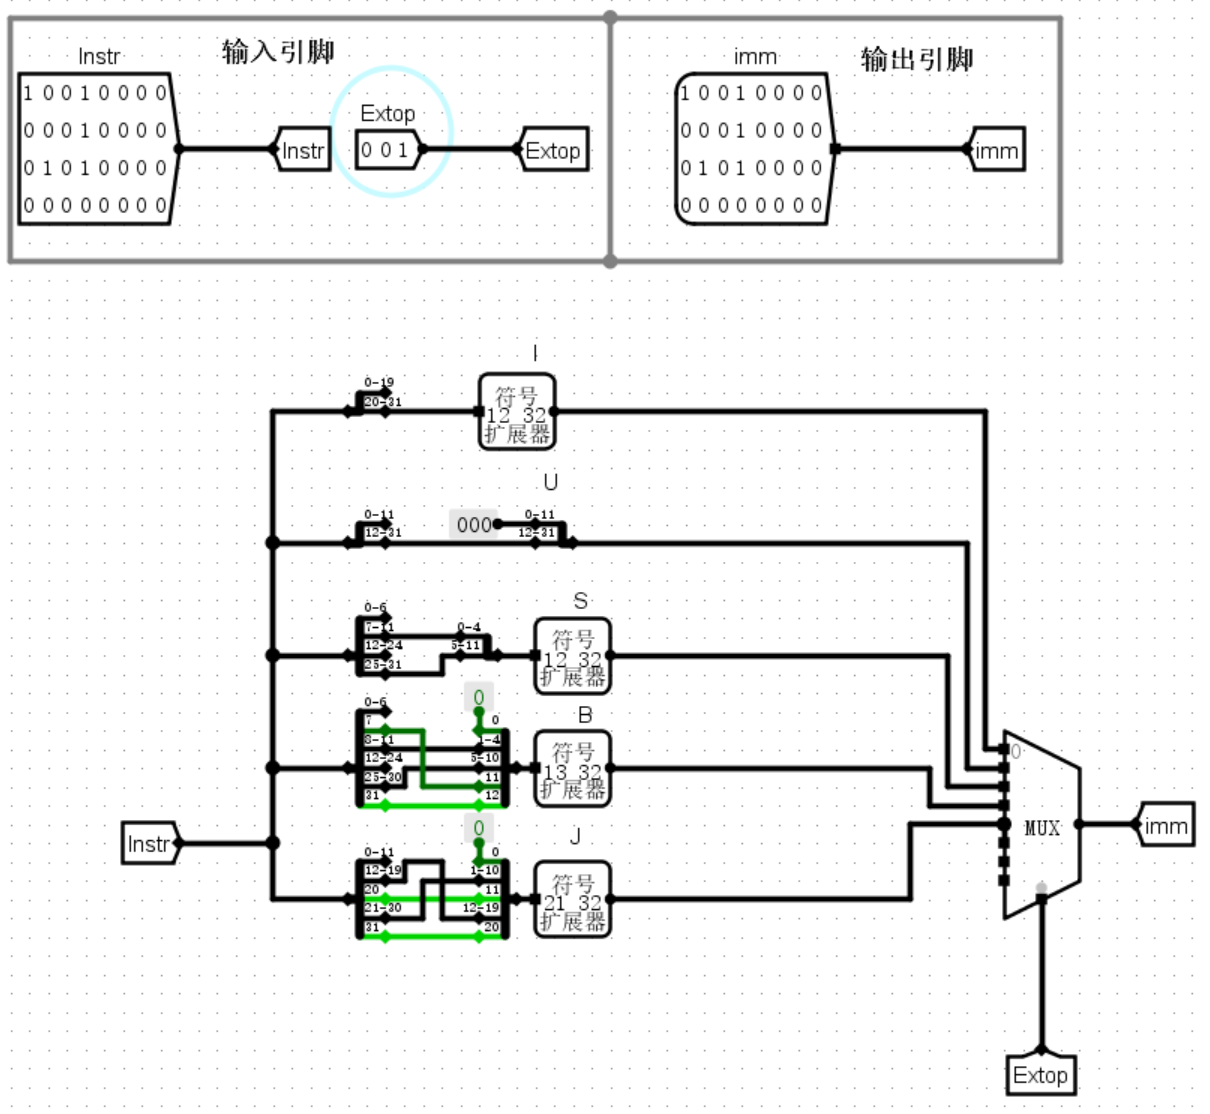
\includegraphics[width=0.8\textwidth]{4.5.2.png}
    \caption{立即数扩展器仿真测试图}
    \end{figure}

    \begin{figure}[H]
        \centering
        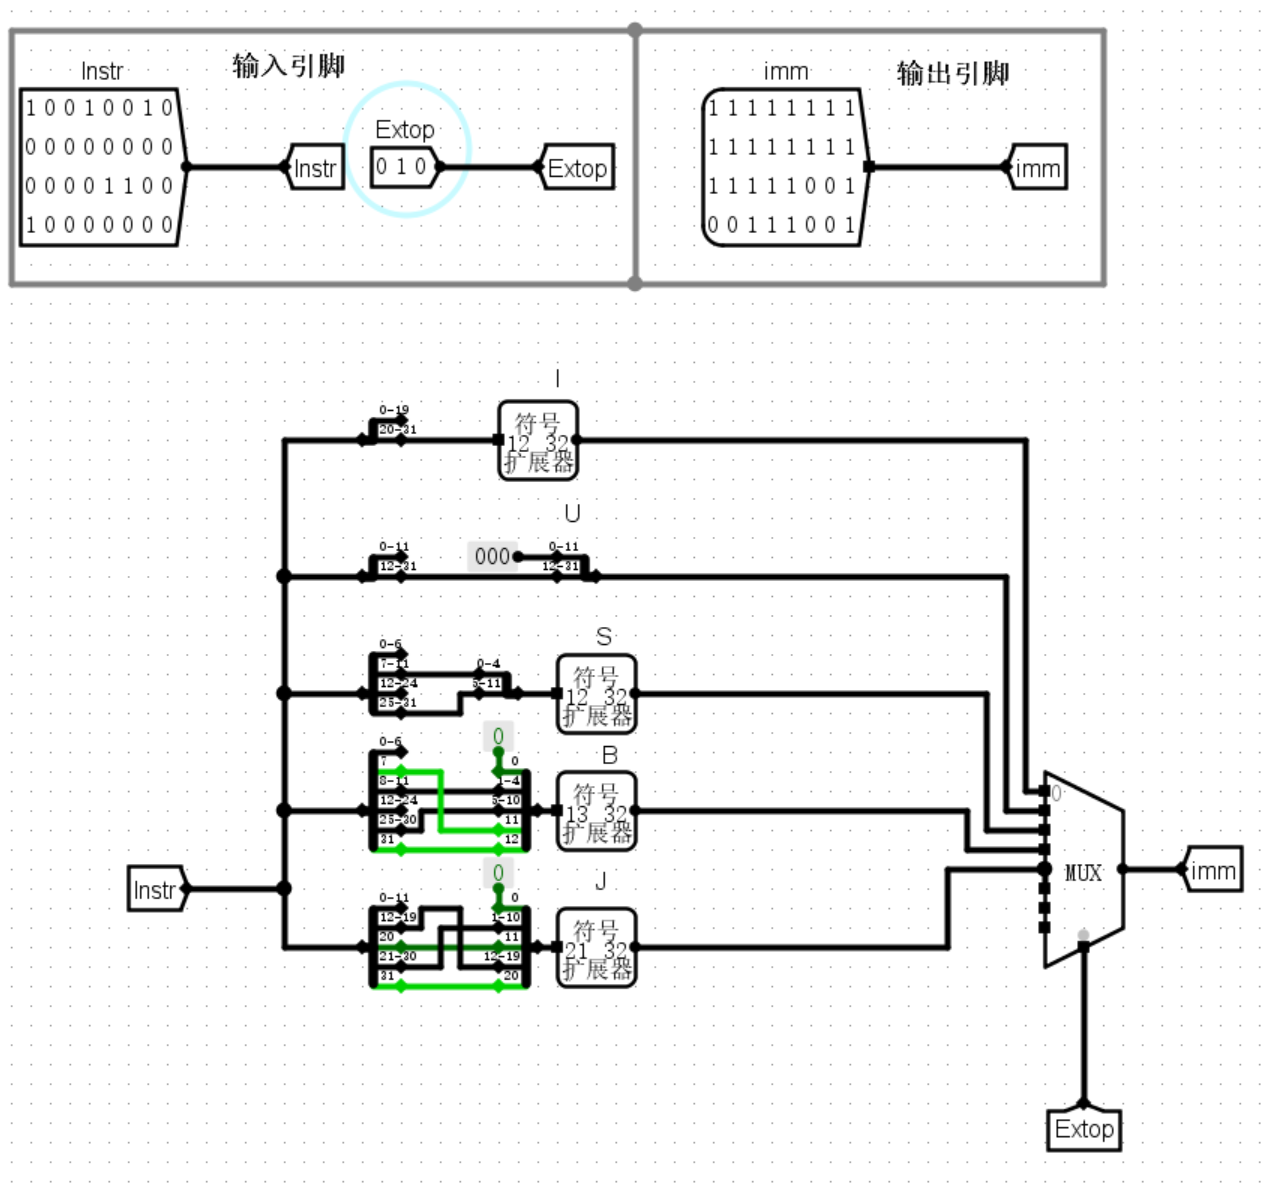
\includegraphics[width=0.8\textwidth]{4.5.3.png}
        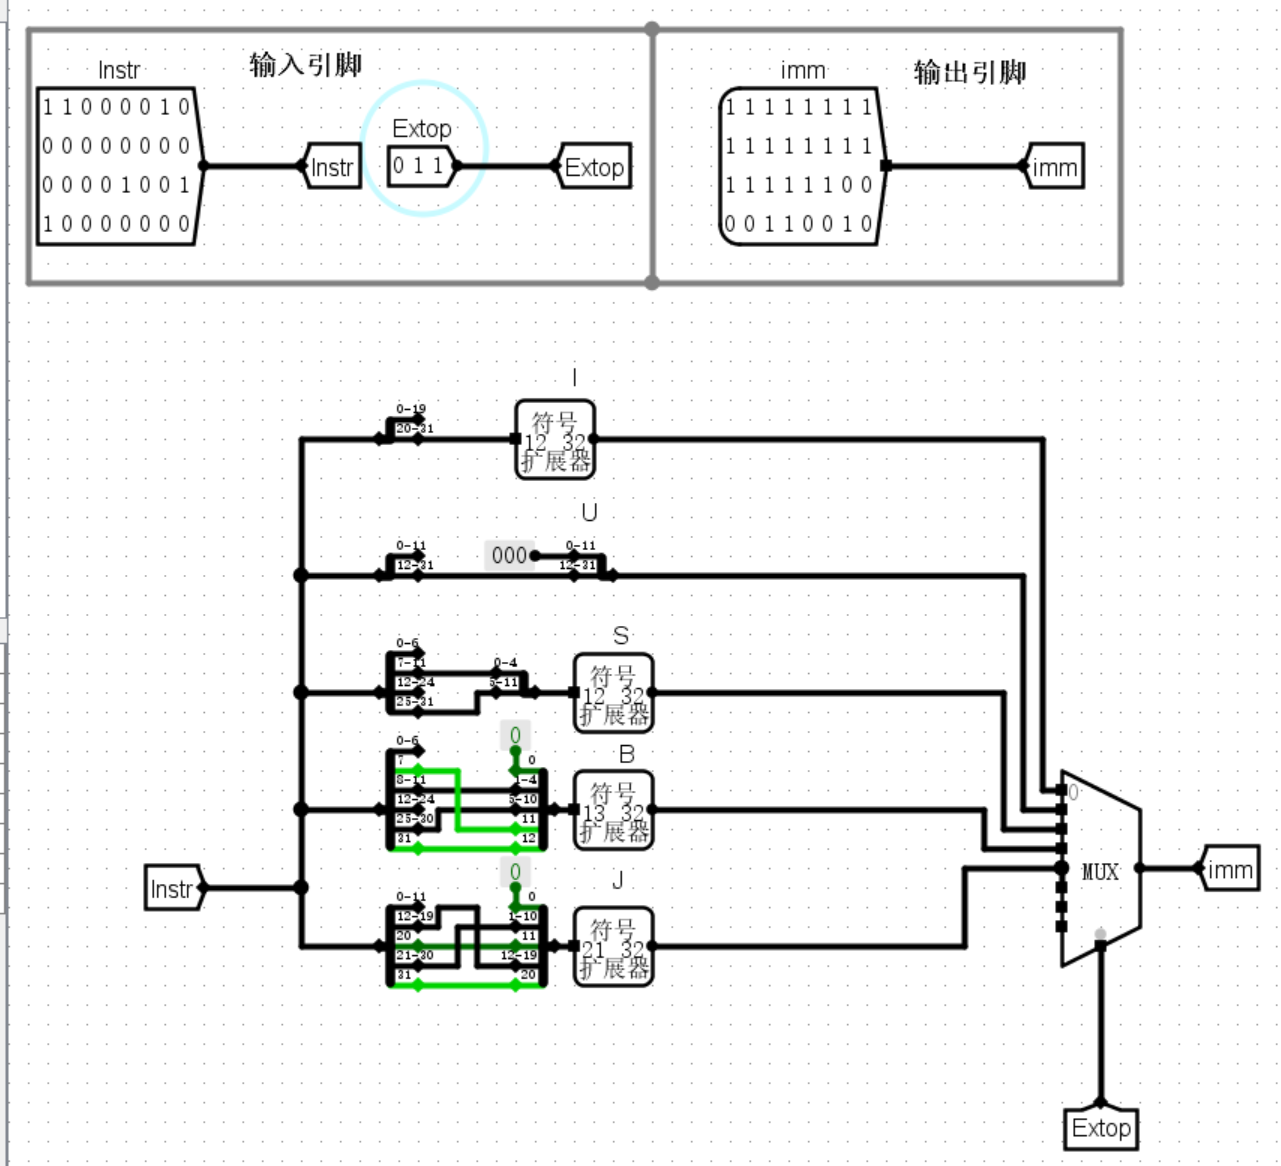
\includegraphics[width=0.8\textwidth]{4.5.4.png}
        \caption{立即数扩展器仿真测试图}
    \end{figure}
    四张图对应了I-type、U-type、S-type、B-type的扩展。所有仿真结果与预期相符。
    
    \subsubsection{错误现象及分析}
    在完成实验的过程中,没有遇到任何错误。

    \subsection{跳转控制器}
    \subsubsection{整体方案设计}

    \begin{figure}[H]
    \centering
    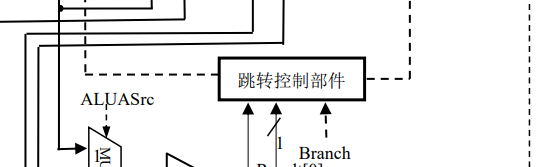
\includegraphics[width=0.8\textwidth]{5.1.png}
    \caption{跳转控制器整体方案设计}
    \end{figure}

    \subsubsection{顶层模块设计}
    实验电路较为简单,不需要顶层模块设计图。

    \subsubsection{引脚作用}
    \begin{table}[H]
    \centering
    \begin{tabular}{|c|c|}
        \hline
        Branch[2:0]     & 输入的 Branch 控制信号 \\ \hline
        Zero   & 输入的 ALU 输出 Zero \\ \hline
        Result0 & 输入的 ALU 输出 Result 信号最低位 \\ \hline
        NxtASrc  & 输出的 NxtASrc 信号 \\ \hline
        NxtBSrc & 输出的 NxtBSrc 信号 \\ \hline
    \end{tabular}
    \caption{跳转控制器引脚作用}
    \end{table}

    \begin{figure}[H]
        \centering
        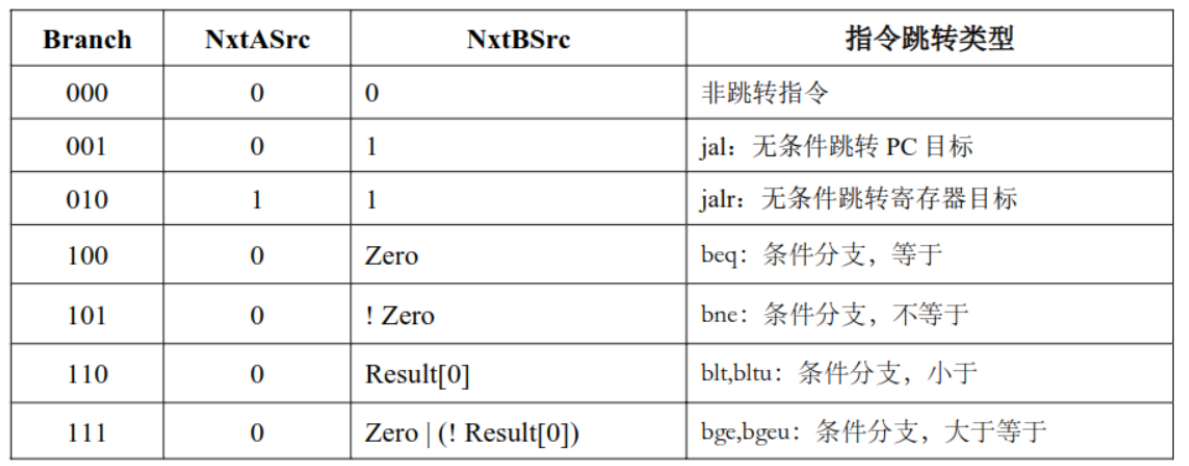
\includegraphics[width=0.8\textwidth]{5.2.png}
        \caption{Branch 控制信号的具体定义}
    \end{figure}

    \subsubsection{原理图和电路图}
    原理图略,实现逻辑函数即可,电路图中使用 MUX 实现。

    \begin{figure}[H]
    \centering
    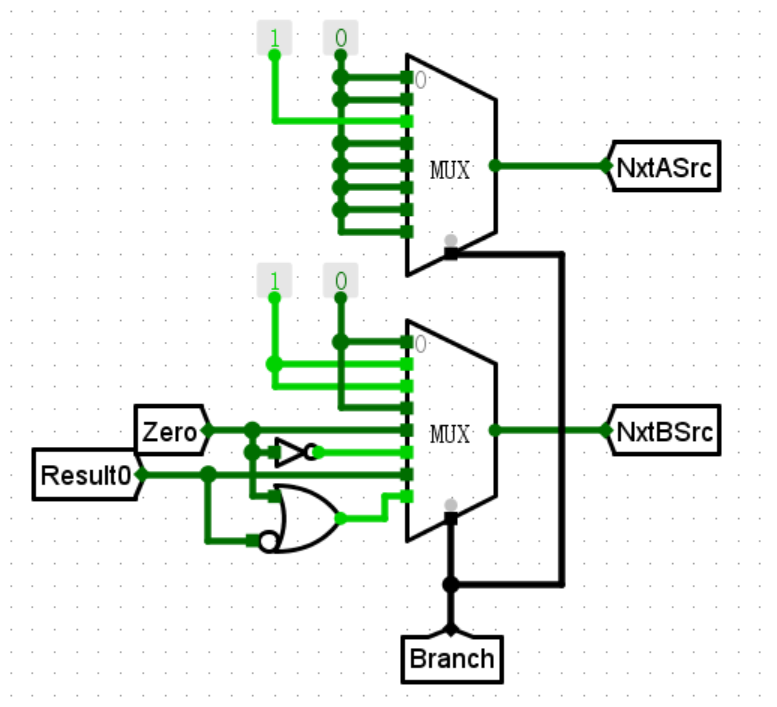
\includegraphics[width=0.8\textwidth]{5.4.png}
    \caption{跳转控制器电路图}
    \end{figure}

    \subsubsection{仿真测试图}
    \begin{figure}[H]
    \centering
    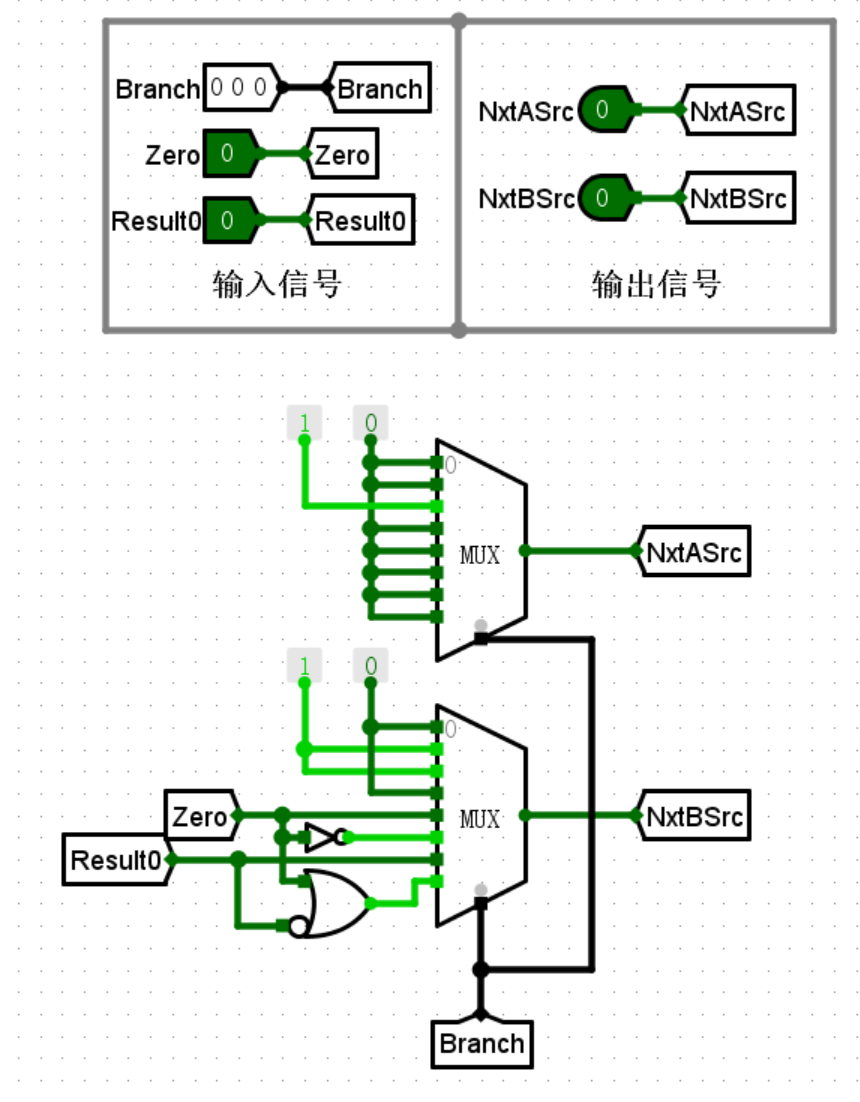
\includegraphics[width=0.8\textwidth]{5.5.1.png}
    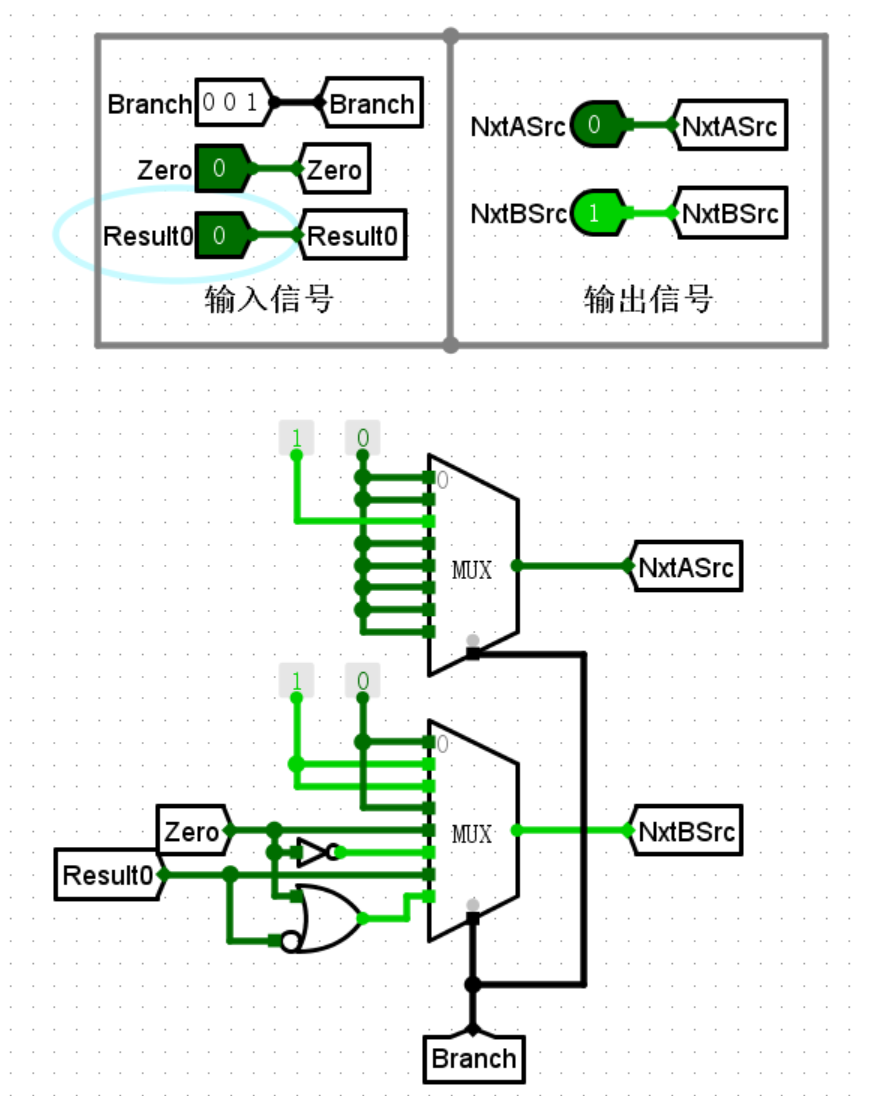
\includegraphics[width=0.8\textwidth]{5.5.2.png}    
    \caption{跳转控制器仿真测试图}
    \end{figure}

    \begin{figure}[H]
        \centering
        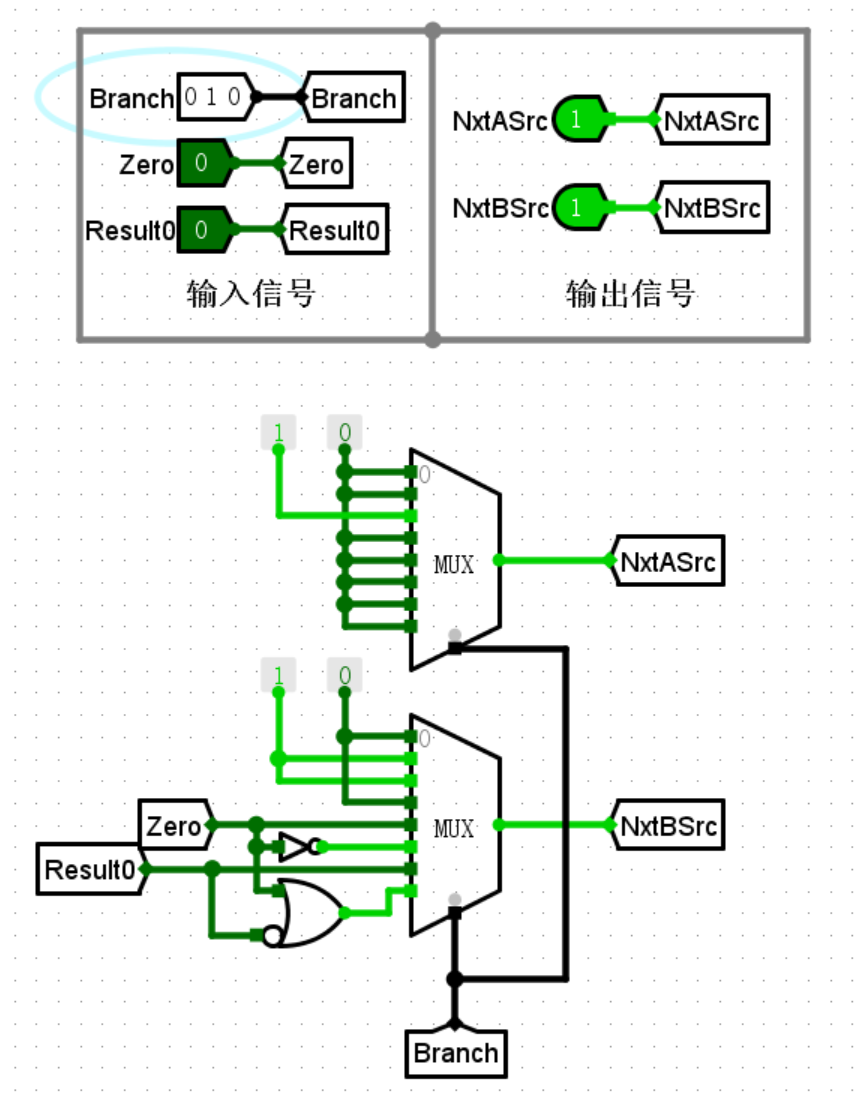
\includegraphics[width=0.8\textwidth]{5.5.3.png}
        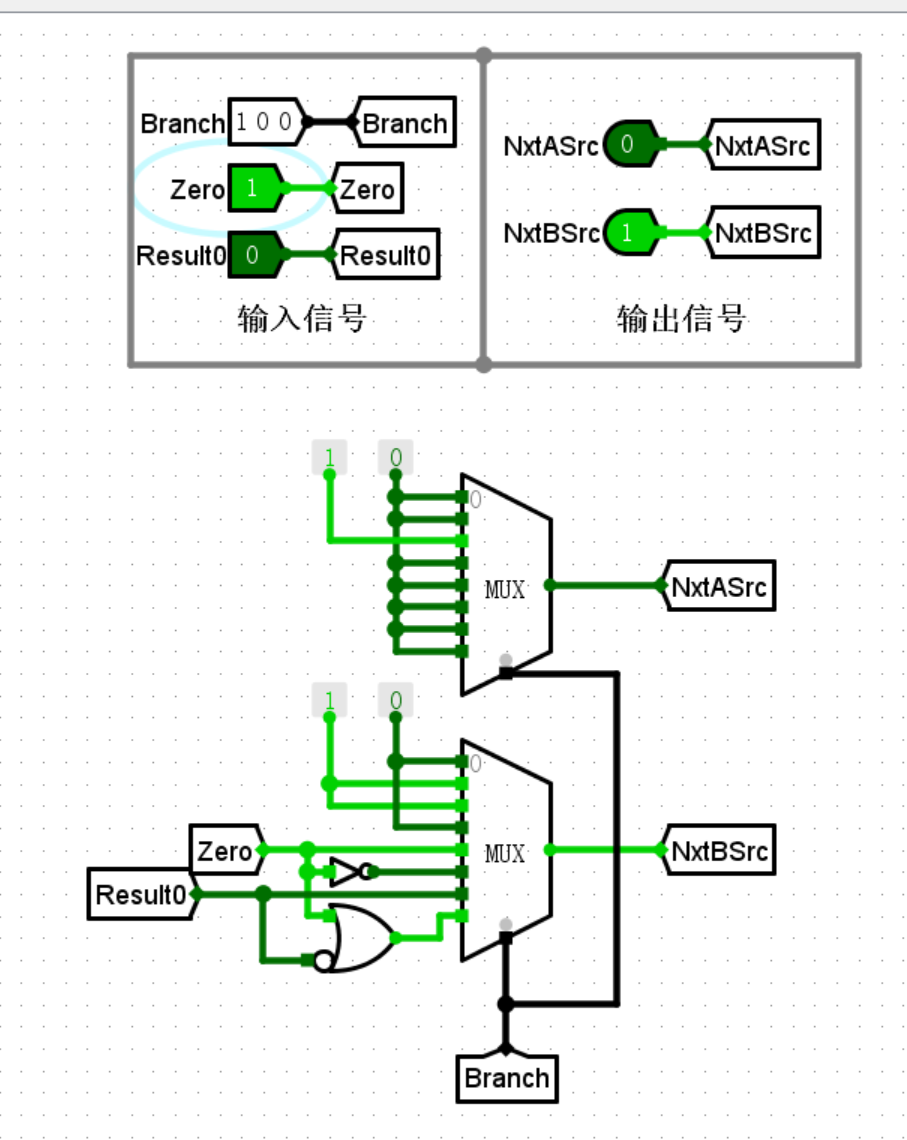
\includegraphics[width=0.8\textwidth]{5.5.4.png}    
        \caption{跳转控制器仿真测试图}
    \end{figure}

    \begin{figure}[H]
        \centering
        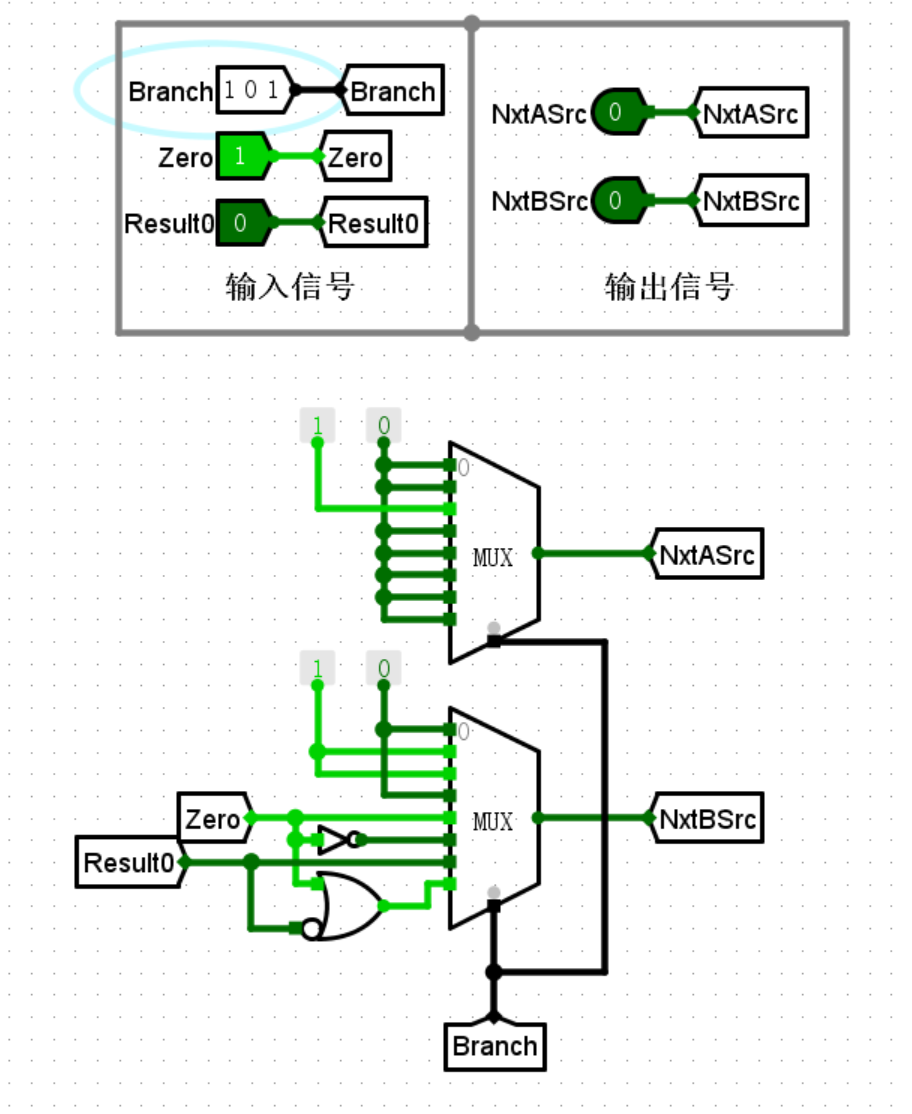
\includegraphics[width=0.8\textwidth]{5.5.5.png}
        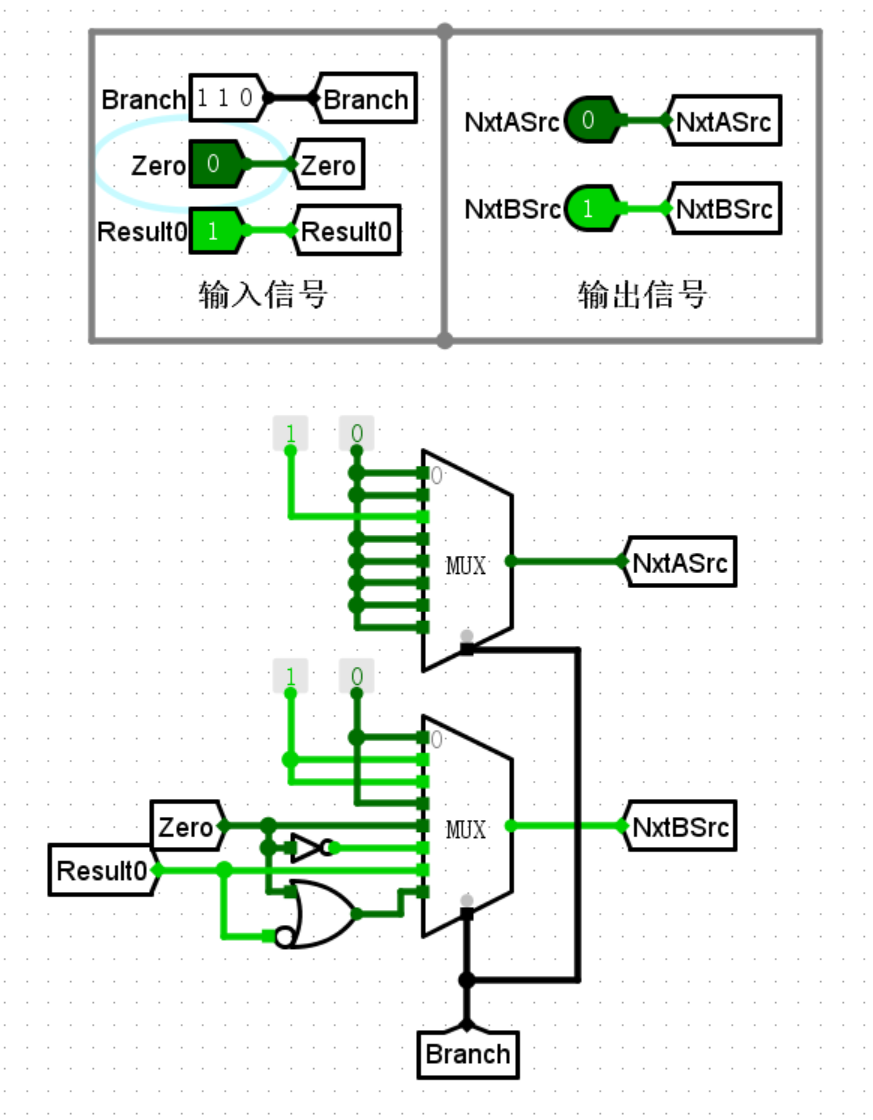
\includegraphics[width=0.8\textwidth]{5.5.6.png}    
        \caption{跳转控制器仿真测试图}
    \end{figure}

    \begin{figure}[H]
        \centering
        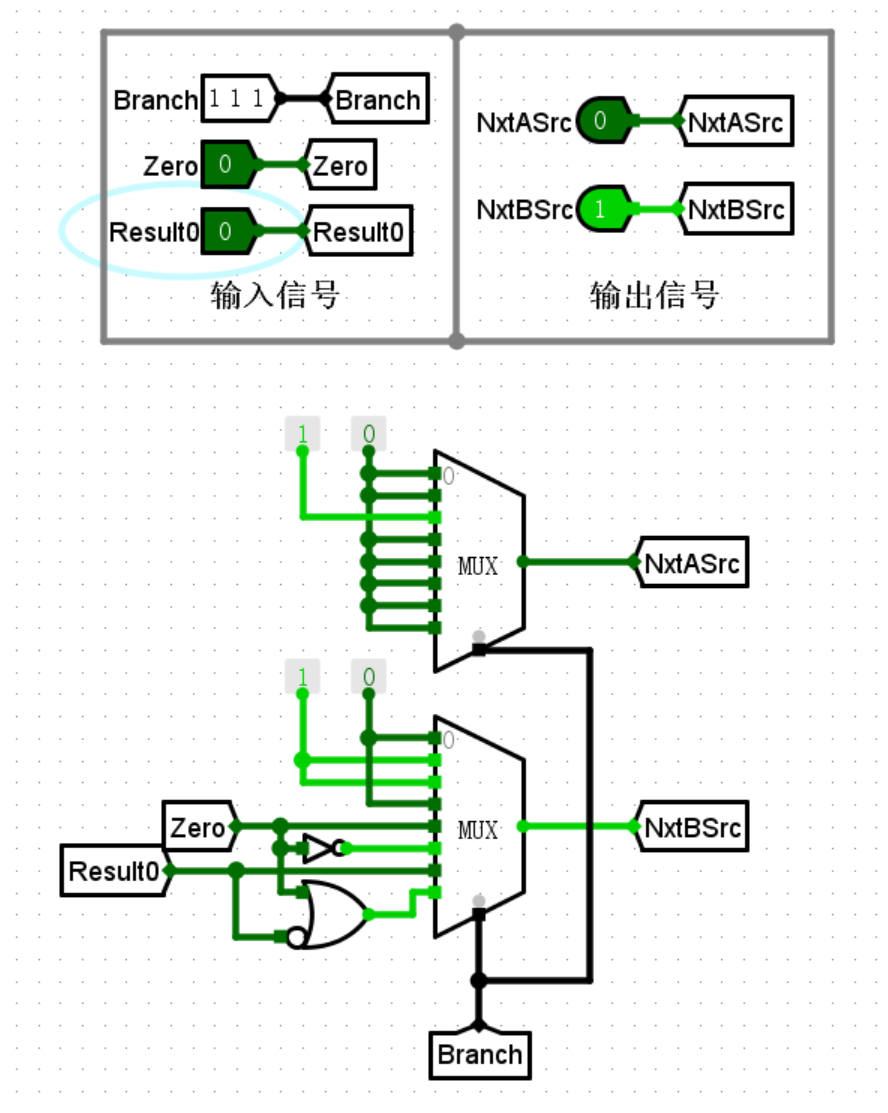
\includegraphics[width=0.8\textwidth]{5.5.7.png}   
        \caption{跳转控制器仿真测试图}
    \end{figure}    
    七张图分别对应于七种 Branch 控制信号的情况,所有仿真结果与预期相符。

    \subsubsection{错误现象及分析}
    在完成实验的过程中,没有遇到任何错误。

    \subsection{IDU}
    \subsubsection{整体方案设计}
    \begin{figure}[H]
    \centering
    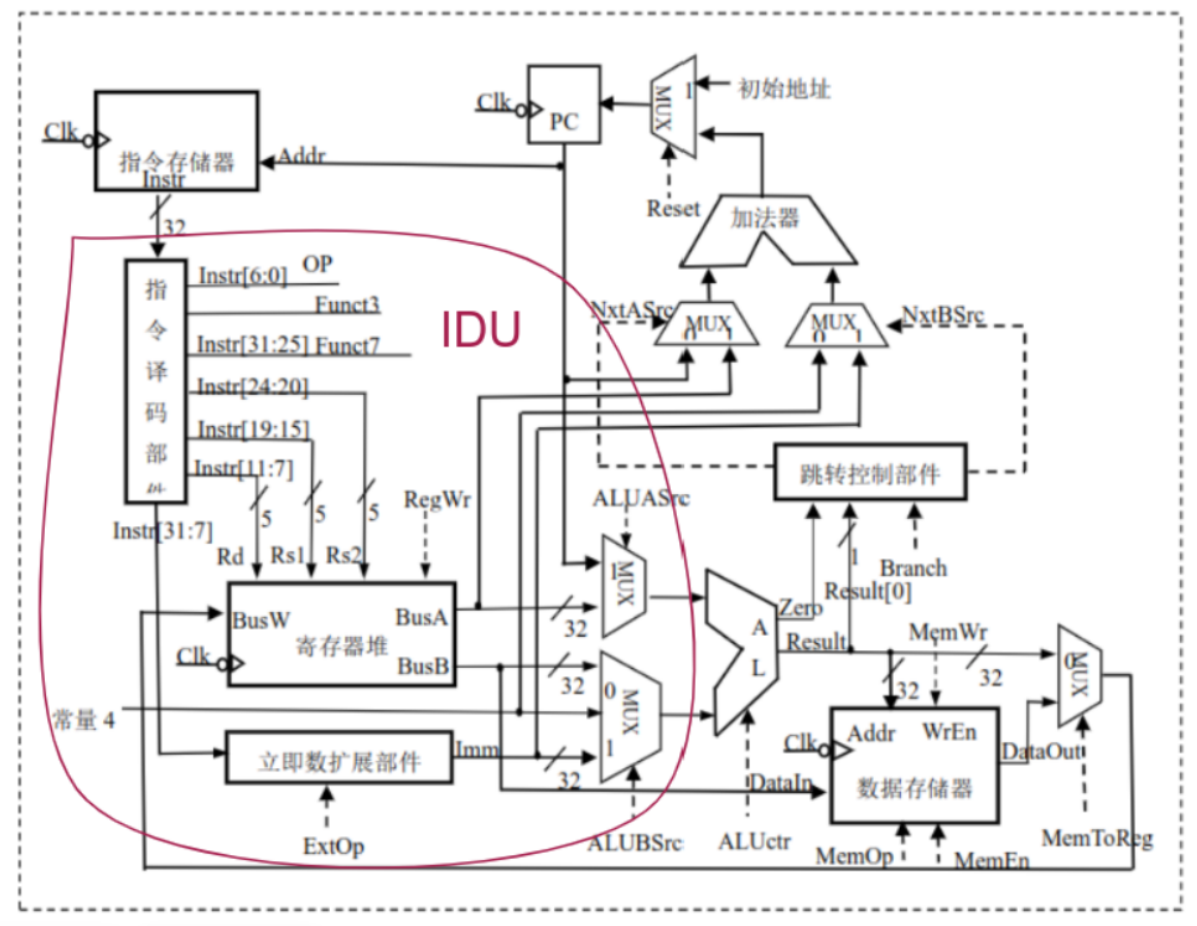
\includegraphics[width=0.8\textwidth]{6.1.png}
    \caption{IDU 整体方案设计}
    \end{figure}

    \subsubsection{顶层模块设计}
    实验电路较为简单,不需要顶层模块设计图。

    \subsubsection{引脚作用}
    \begin{table}[H]
    \centering
    \begin{tabular}{|c|c|}
        \hline
        IR[31:0]      & 输入的指令 \\ \hline
        PC[31:0]    & 输入的 PC \\ \hline
        BusW[31:0]  & 输入的寄存器堆写入数据 \\ \hline
        Clk  & 输入的时钟信号,上升沿有效 \\ \hline
        ExtOp[2:0]  & 输入的立即数扩展方式 \\ \hline
        RegWr & 输入的寄存器堆写使能信号 \\ \hline
        ALUASrc & 输入的 ALU 第一个操作数选择信号 \\ \hline
        ALUBSrc[1:0]  & 输入的 ALU 第二个操作数选择信号 \\ \hline
        OP[6:0]  & 输出的指令操作码 \\ \hline
        Func3[2:0], Func7[6:0] & 输出的指令功能码   \\ \hline
        Imm[31:0] & 输出的立即数 \\ \hline
        BusA[31:0] & 输出的 R[rs1],用于下地址逻辑 \\ \hline
        DataIn[31:0] & 输出的 R[rs2],用于写入数据存储器 \\ \hline
        DataA[31:0] & 输出的 ALU 第一个操作数 \\ \hline
        DataB[31:0]  & 输出的 ALU 第二个操作数 \\ \hline
    \end{tabular}
    \caption{IDU引脚作用}
    \end{table}
    
    \subsubsection{原理图和电路图}
    原理图同整体方案设计图,电路图如下。

    \begin{figure}[H]
    \centering
    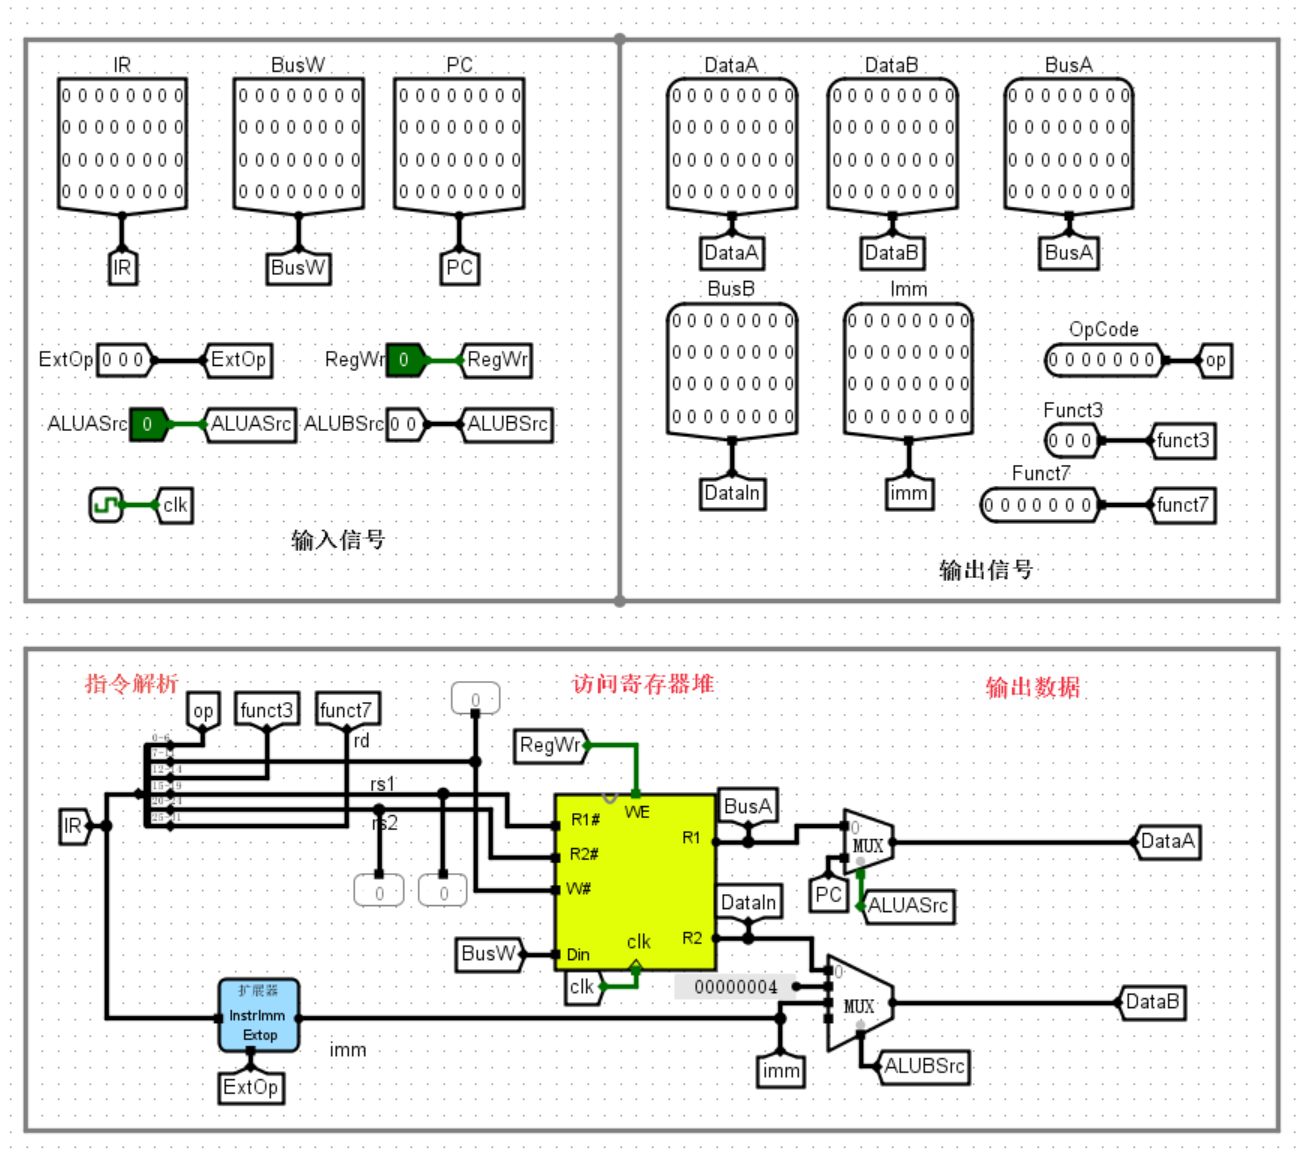
\includegraphics[width=0.8\textwidth]{6.4.2.png}
    \caption{IDU 电路图}
    \end{figure}

    \subsubsection{仿真测试图}
    \begin{figure}[H]
    \centering
    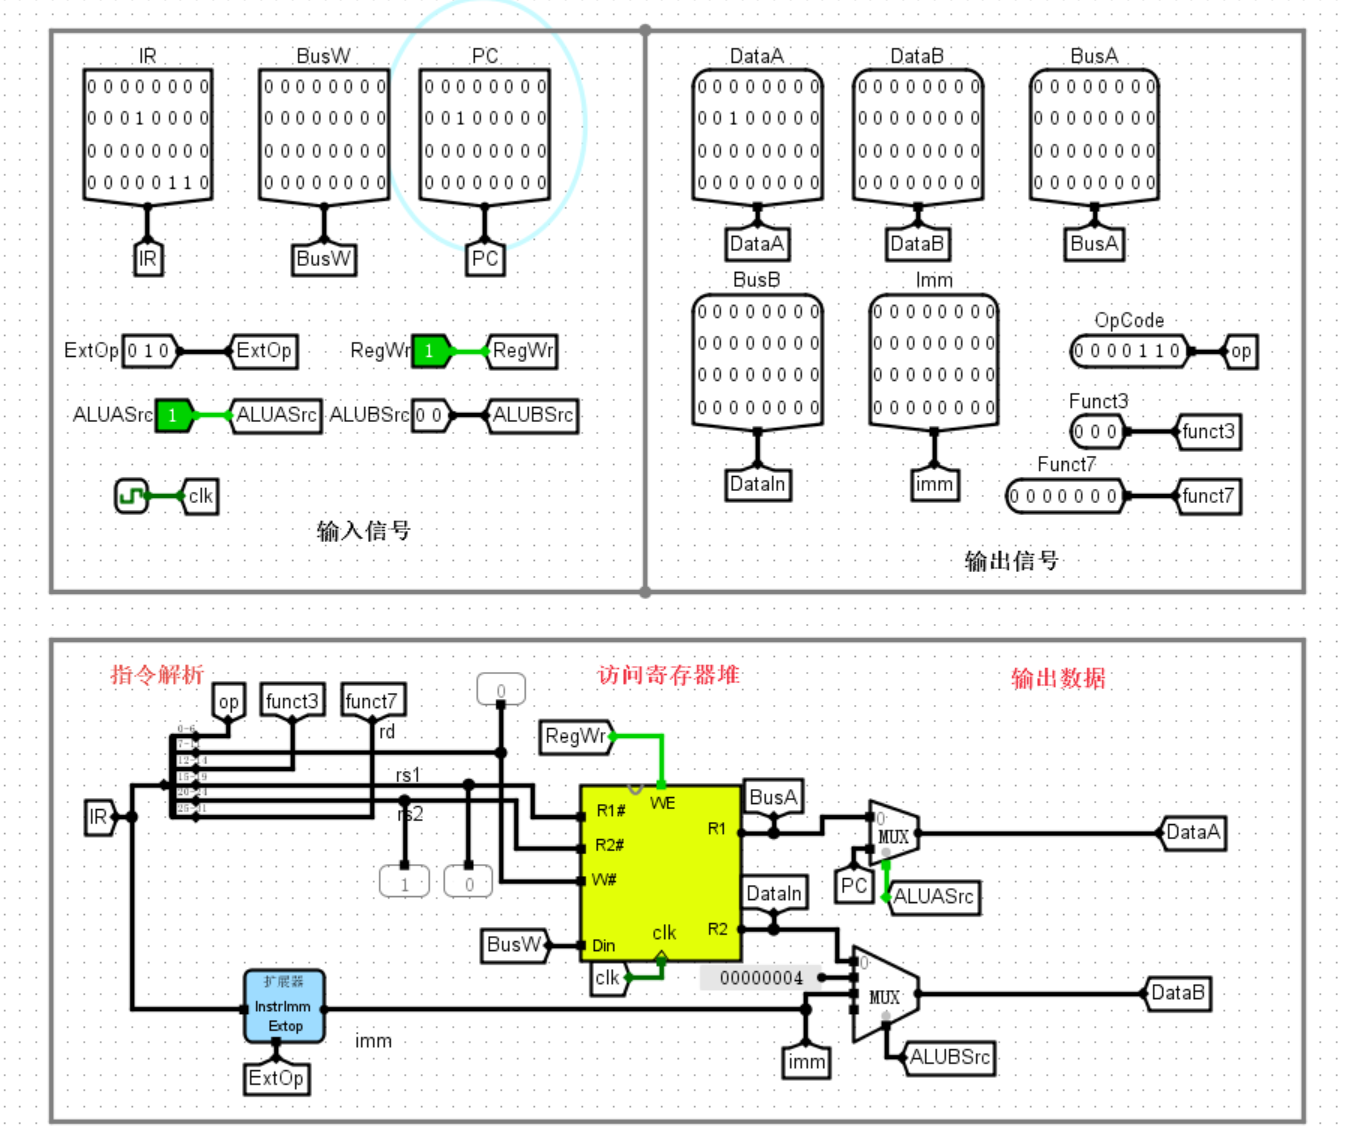
\includegraphics[width=0.8\textwidth]{6.5.1.png}
    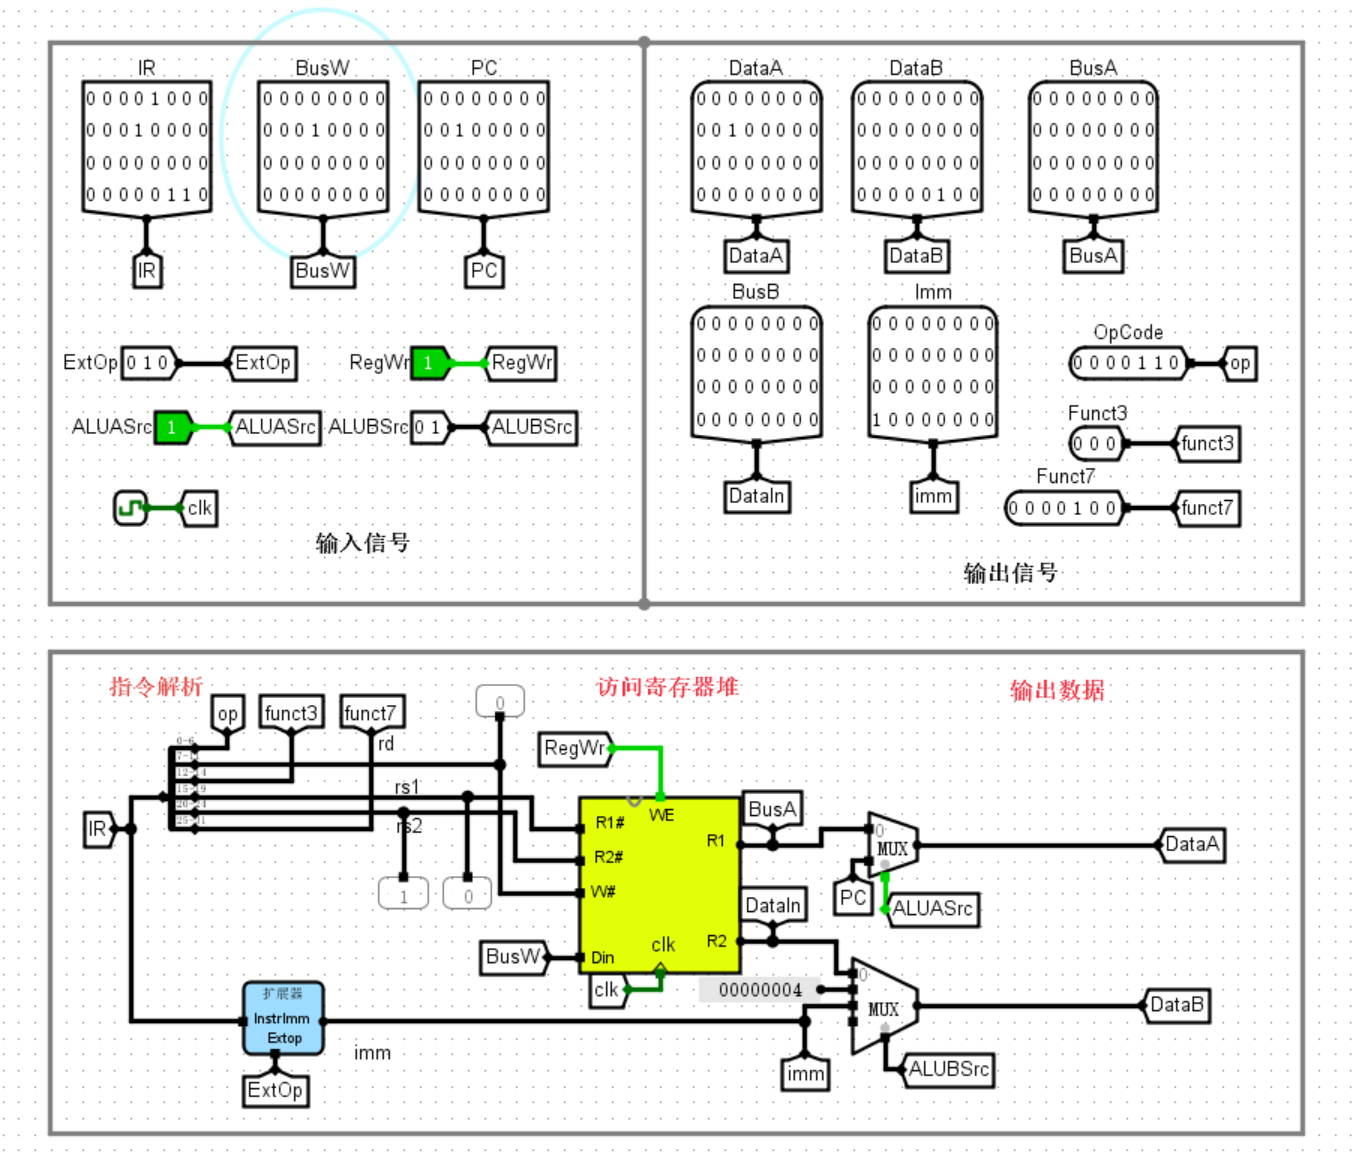
\includegraphics[width=0.8\textwidth]{6.5.2.png}
    \caption{IDU 仿真测试图}
    \end{figure}

    展示前两个指令,仿真测试图留到数据通路完成后进行自动化测试。

    \subsubsection{错误现象及分析}
    在完成实验的过程中,没有遇到任何错误。

    \subsection{数据通路}
    \subsubsection{整体方案设计}
    \begin{figure}[H]
    \centering
    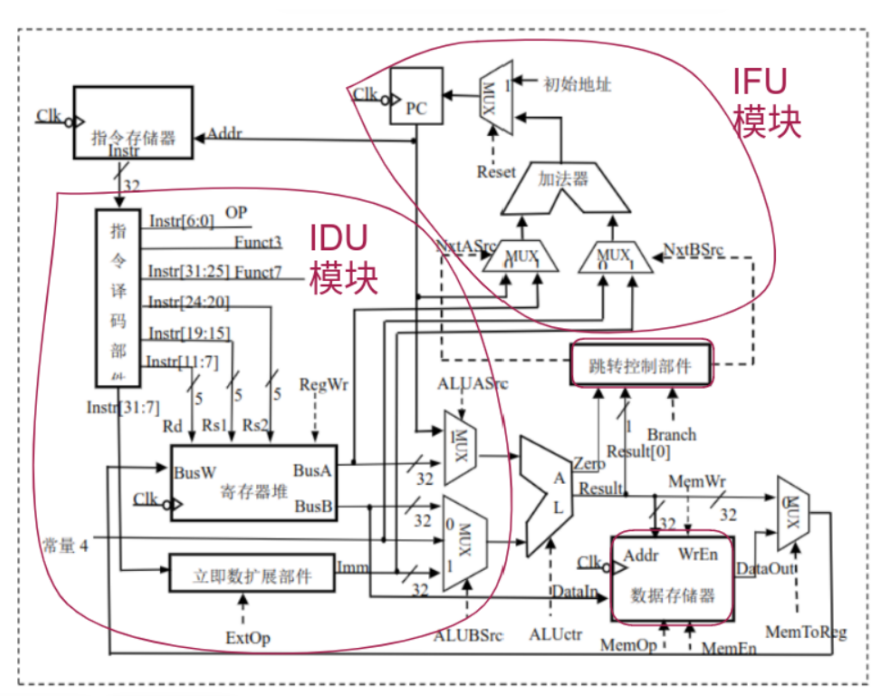
\includegraphics[width=0.8\textwidth]{7.1.png}
    \caption{数据通路 整体方案设计}
    \end{figure}

    \subsubsection{引脚作用}
    \begin{figure}[H]
        \centering
        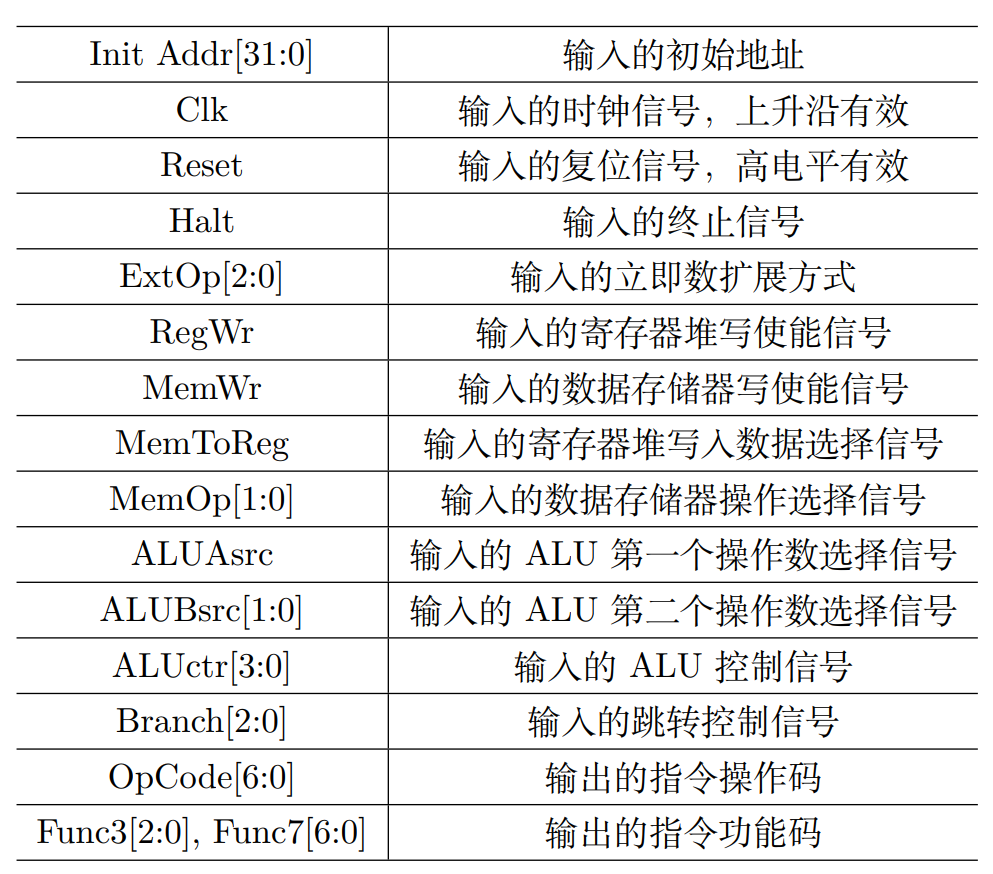
\includegraphics[width=0.8\textwidth]{7.2.png}
        \caption{数据通路 引脚作用}
    \end{figure}

    \subsubsection{原理图和电路图}
    原理图同整体方案设计图,电路图如下。

    \begin{figure}[H]
    \centering
    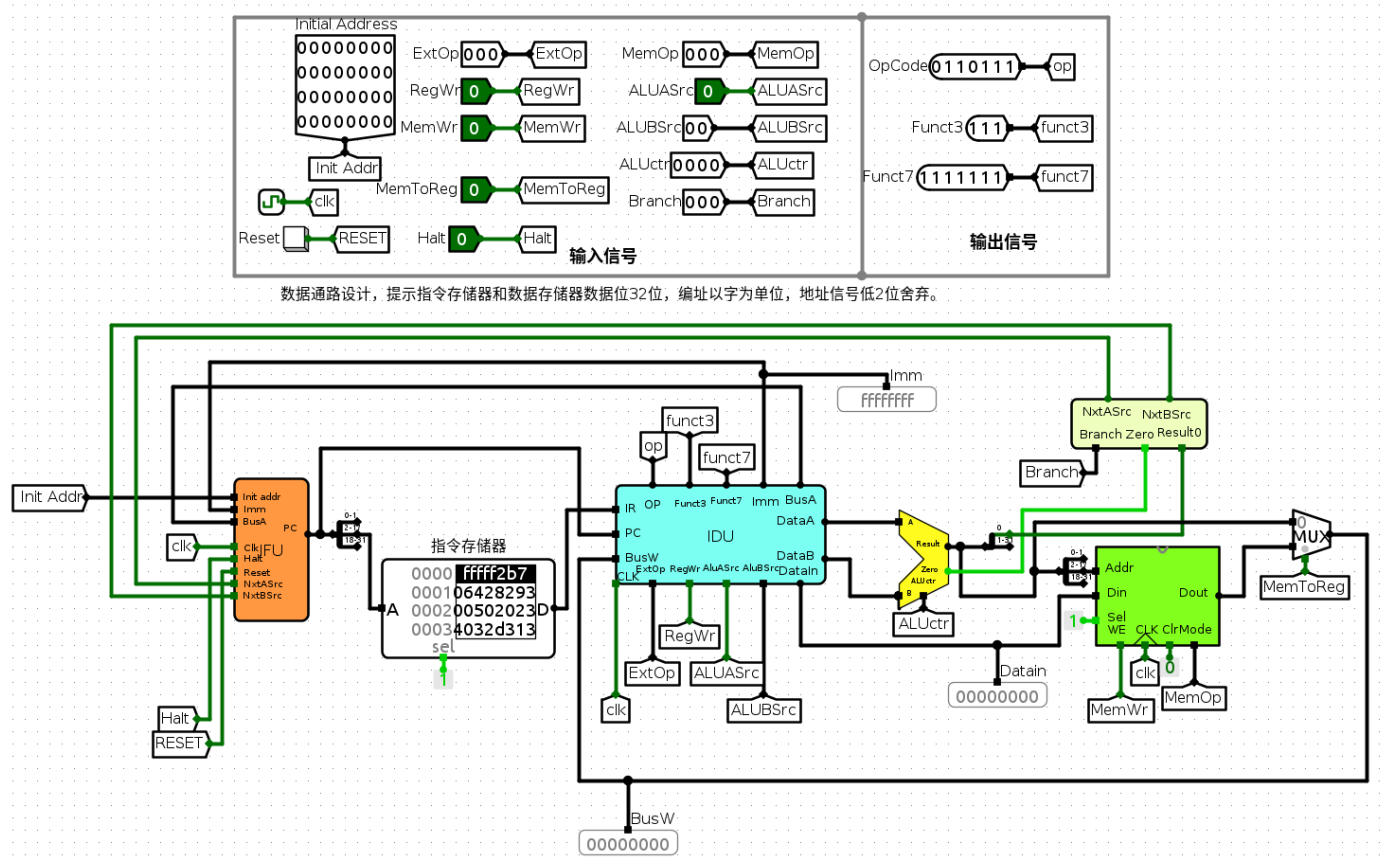
\includegraphics[width=0.8\textwidth]{7.4.2.png}
    \caption{数据通路 电路图}
    \end{figure}

    \subsubsection{仿真测试图}
    在数据存储器中输入表中一系列指令:fffff2b7、06428293、00502023...\\
    结果正确。经过仿真,完整的测试表如下表和下图(电路中regfile存储信息)所示。
    \begin{figure}[H]
        \centering
        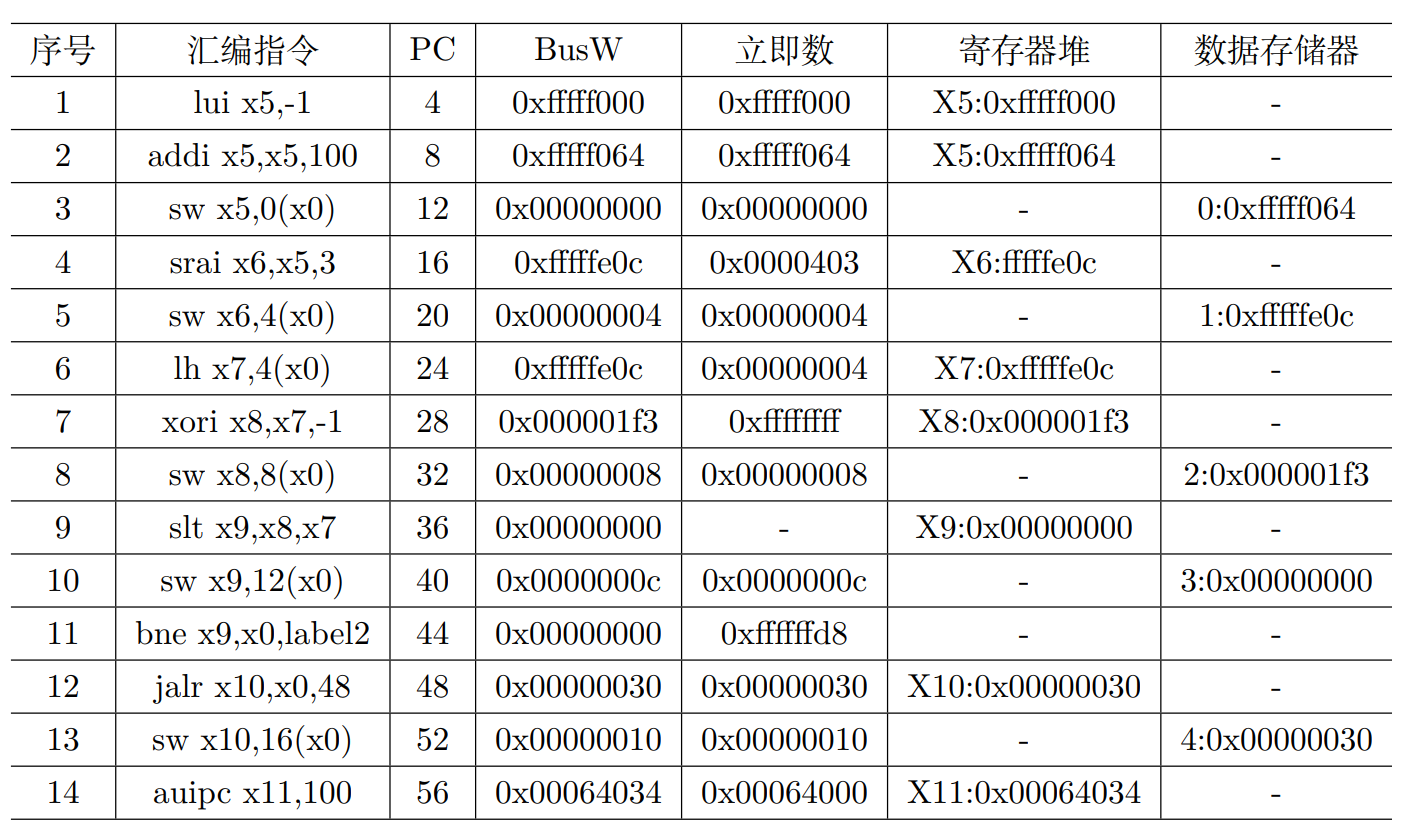
\includegraphics[width=0.8\textwidth]{7.5.png}
        \caption{数据通路 测试表}
    \end{figure}

    \begin{figure}[H]
        \centering
        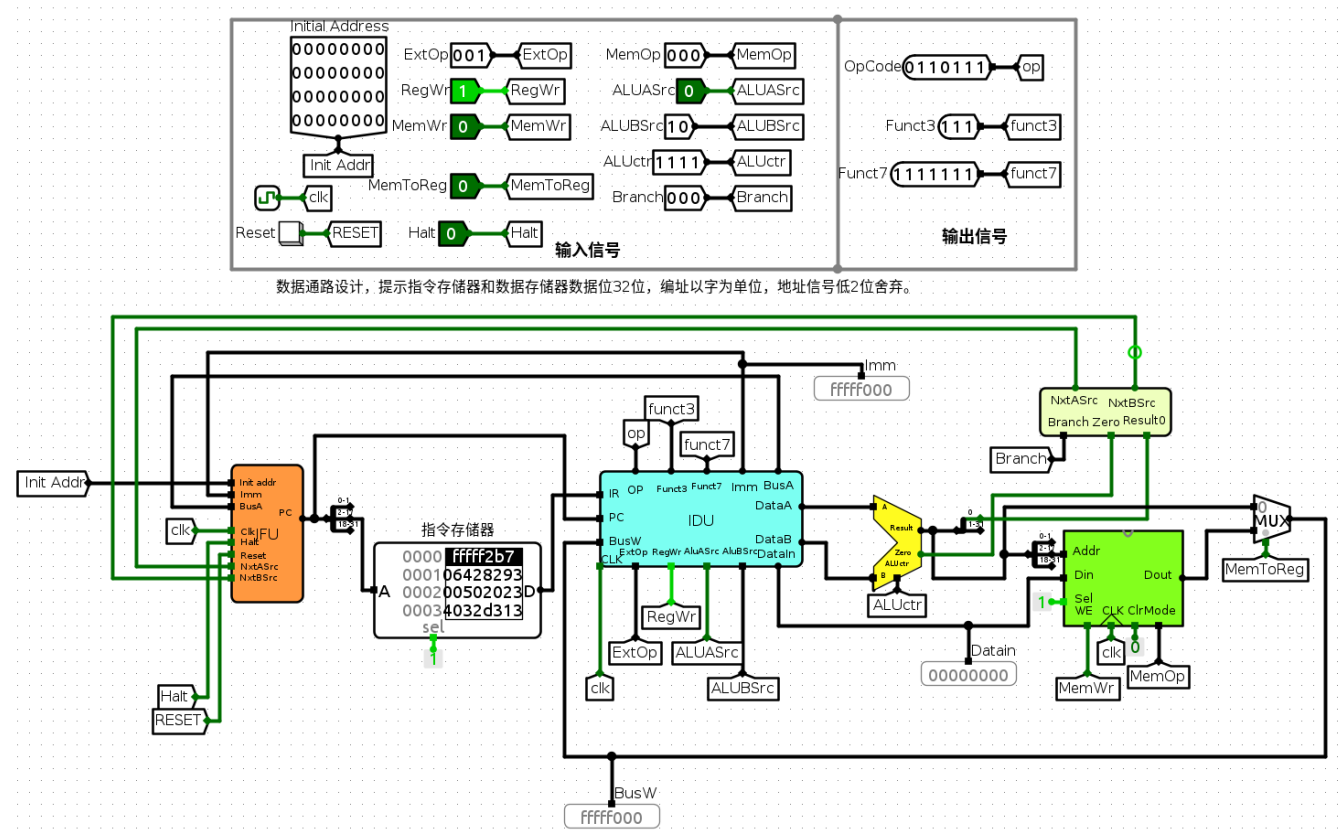
\includegraphics[width=0.4\textwidth]{7.5.1.png}
        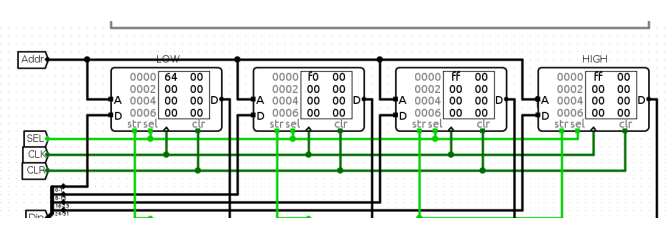
\includegraphics[width=0.4\textwidth]{7.5.2.png}
        \caption{数据通路 测试图}
    \end{figure}

    \begin{figure}[H]
        \centering
        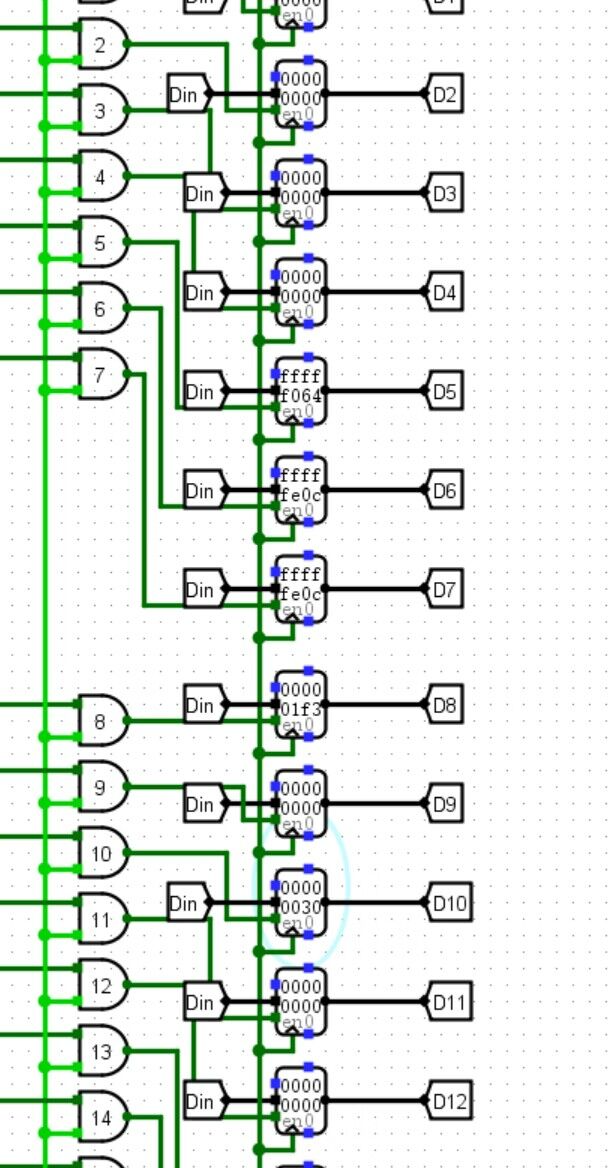
\includegraphics[width=0.4\textwidth]{7.5.3.png}
        \caption{数据通路 regfile存储信息}
    \end{figure}

    \subsubsection{错误现象及分析}
    在完成实验的过程中,没有遇到任何错误。

    \section{思考题}


    \subsection{如何拓展 ROM 实验实现跑马灯的功能,在 3 个 LED 点阵中,滚动显示 5 个 ASCII 字符,如“NJUCS”。}
    可以使用一个模五计数器配合 MUX 实现 ASCII 码的轮换,每个时钟信号,模五计数器加一,然后将其输出与 MUX 的选择信号相连,在三个MUX中轮流选择NJU,JUC,UCS,...这样就可以实现跑马灯的效果。
    \begin{figure}[H]
        \centering
        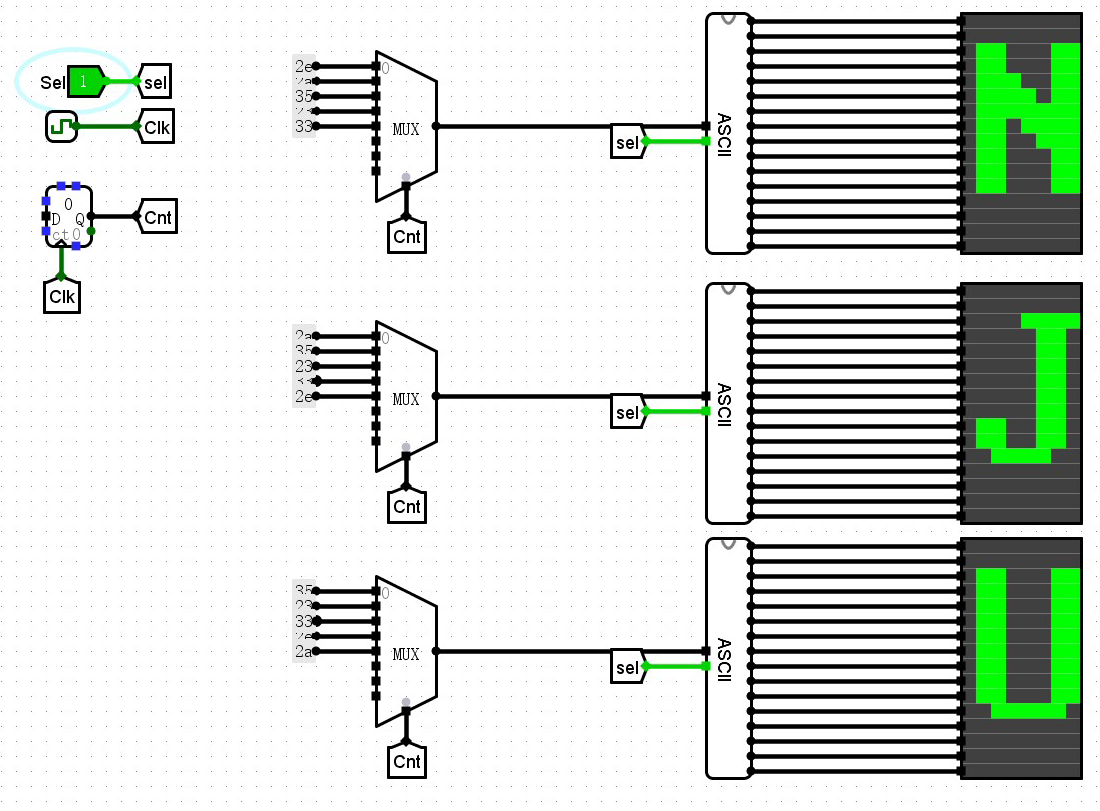
\includegraphics[width=0.4\textwidth]{8.1.png}
        \caption{跑马灯}
    \end{figure}
    \begin{figure}[H]
        \centering
        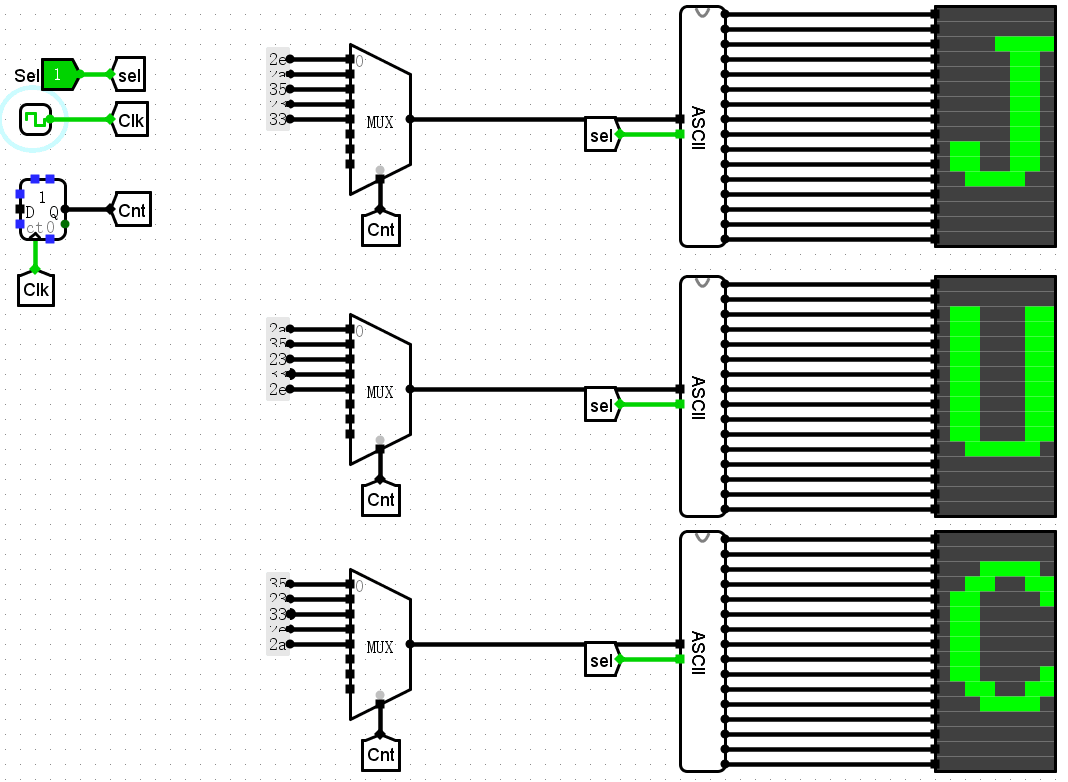
\includegraphics[width=0.4\textwidth]{8.2.png}
        \caption{跑马灯}
    \end{figure}
    \begin{figure}[H]
        \centering
        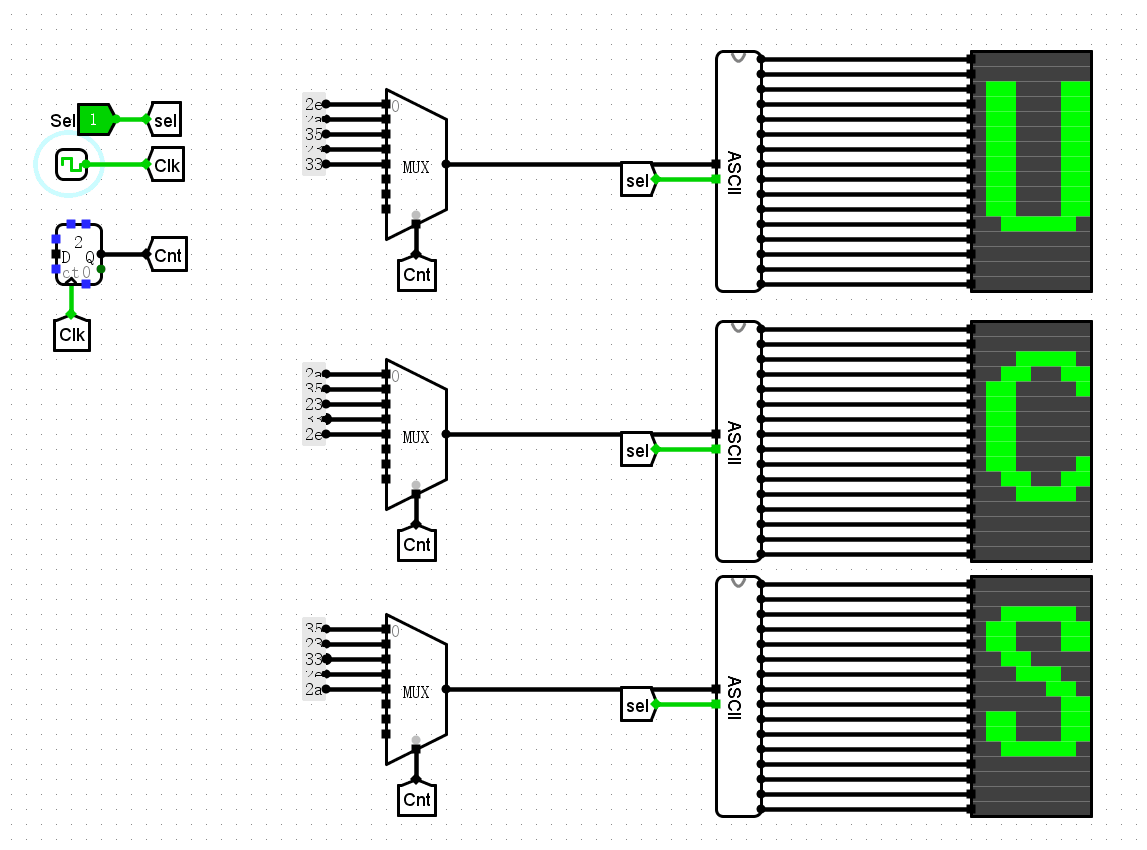
\includegraphics[width=0.4\textwidth]{8.3.png}
        \caption{跑马灯}
    \end{figure}

    \subsection{表 5.2 给出的第 11 条测试指令中标号 label2 所表示的偏移地址是多少(用真值表示)?}
    label2 表示的偏移值0xffffffd8,真值为 -0x00000028,即 -40。


    \subsection{在 Risc-V 架构中,举例说明什么是伪指令?伪指令如何实现?}
    伪指令是在汇编语言中提供的一种不是本身即可执行的指令,而是被解释器(汇编器)用来简化汇编代码或提高可读性的语句。Risc-V 中的伪指令是一些类似于指令但实际上却不会在硬件中被执行的操作。例如,Risc-V 中包含的伪指令 .word,可以让汇编器将一个 32 位的值存储到程序的某个位置。而 .byte 则可以将一个 8 位的值存储到程序的某个位置。\par
    实现伪指令的主要方法是将伪指令转换为真正的指令序列,这个任务由汇编器负责。例如,.word 伪指令可以转换为几条真正的指令序列,包括 lui(将高 20 位的立即数存入寄存器),addi(将低 12 位的立即数加入寄存器)等等。这些指令的作用是将一个 32 位的立即数存放到指定的内存位置上。因此,当程序被加载到内存中时,这些指令会被正确地翻译成相应的机器指令,在硬件中最终被执行。


    \subsection{在指令执行过程中,如何实现程序结束后,指令不再继续执行?}
    在程序的结尾添加一个无限循环指令,使程序执行完成后陷入一个无限循环中,从而停止执行。例如,在 RISC-V 中,可以使用一个 j(跳转)指令来无限循环,如 j .(跳转到当前地址)或 j label(跳转到标签 label 处)。

\end{document}